\documentclass[11pt]{article}

%\usepackage{gb4e}
%\usepackage{pslatex}
\usepackage{apacite}
\usepackage{amsmath,amssymb}
\usepackage{graphicx}
\usepackage{color}
\usepackage{url}
\usepackage{fullpage}
\usepackage{setspace}
\usepackage{booktabs}
\usepackage{lingmacros}

%\newcommand{\url}[1]{$#1$}

\definecolor{Blue}{RGB}{50,50,200}
\newcommand{\blue}[1]{\textcolor{Blue}{#1}}

\definecolor{Red}{RGB}{255,0,0}
\newcommand{\red}[1]{\textcolor{Red}{#1}}
\newcommand{\jd}[1]{\textcolor{Red}{[jd: #1]}} 

\definecolor{Green}{RGB}{50,200,50}
\newcommand{\ndg}[1]{\textcolor{Green}{[ndg: #1]}}  

 \newcommand{\denote}[1]{\mbox{ $[\![ #1 ]\!]$}}


\newcommand{\subsubsubsection}[1]{{\em #1}}
\newcommand{\eref}[1]{(\ref{#1})}
\newcommand{\tableref}[1]{Table \ref{#1}}
\newcommand{\figref}[1]{Figure \ref{#1}}
\newcommand{\appref}[1]{Appendix \ref{#1}}
\newcommand{\sectionref}[1]{Section \ref{#1}}

%\doublespacing


\title{Wonky worlds: Listeners revise common ground when utterances are odd}
%\title{Wonky worlds: Listeners reconsider world knowledge when utterances are odd}
%Non-sinking marbles are wonky: defeasible world knowledge in language interpretation}

 
\author{{\large \bf Judith Degen, Michael Henry Tessler, Noah D.~Goodman} \\
  \{jdegen,mhtessler,ngoodman\}@stanford.edu\\
  Department of Psychology, 450 Serra Mall \\
  Stanford, CA 94305 USA}

% ggplot colors: "#F8766D", "#A3A500", "#00BF7D", "#E76BF3", "#00B0F6"

% variations on blue: "#007fb1", "#4ecdff"


%% TODO
% somewhere in the intro, discuss what other theories of scalar implicature/utterance interpretation have to say about world knowledge 
% add Exp. 4 (run it first...)
% rework discussion
% add appendix with all items

% in intro (or discussion?) talk about what other people have said about how world knowledge is integrated in utterance interpretation, and data that shows that it does. e.g., from guerts (2010, p. 78) : "In general, a sentence like �The peanut was in love�, would yield a massive N400 for the last word. But what will happen when this sentence is embedded in a discourse like the following: 'A woman saw a dancing peanut who had a big smile on his face. The peanut was singing about a girl he had just met. And judging from the song, the peanut was totally crazy about her. The woman thought it was really cute to see the peanut singing and dancing like that. The peanut was {salted/in love}, and by the sound of it, this was definitely mutual. He was seeing a little almond.' (Nieuwland and van Berkum 2006: 1106) As reported by Nieuwland and van Berkum, in this context it is �salted�, not �in love�, that elicits an N400. Apparently, the expectations tracked by the N400 take into account contextual information, as well as general world knowledge. One of the most salient components of the context is the speaker, and van Berkum et al. (2008) showed that the N400 takes into account information about the speaker, too. In van Berkum et al.�s study, people listened to sen- tences whose meanings might be at odds with reasonable assumptions about the speaker�s sex, age, or social status, as inferred from the speaker�s voice. For example, when �I have a large tattoo on my back� was spoken in an upper- class accent, there was an obvious discrepancy between social elevation and dorsal decoration, which became apparent at the critical word �tattoo�. This type of mismatch, too, turned out to yield an N400."

\begin{document}

\maketitle


\begin{abstract}

Knowledge about the world enters into sentence interpretation in complex ways, and may be defeasible in light of speakers' utterances.  Yet there is to date a surprising lack of systematic investigation into the role of world knowledge in pragmatic inference. In this paper, we show that a state-of-the-art model of pragmatic interpretation greatly overestimates the influence of world knowledge on the interpretation of utterances with quantifier words, like \emph{Some of the marbles sank}. We extend the model to capture the idea that  listeners are uncertain about the background knowledge that speakers are bringing to the conversation, i.e., about what knowledge is in common ground. This extension greatly improves model predictions about listeners' interpretation and also makes good qualitative predictions about listeners' judgments of how likely the world is to be (ab)normal in light of a speaker's statement. \blue{In addition, we show that the diminished effect of world knowledge on pragmatic inference is not attributable to a speaker's perceived lack of cooperativity; systematic lesions to the model simulating reduced speaker cooperativity predict a \emph{greater} effect of world knowledge---a prediction that is borne out empirically.} 
\ndg{say something more clear about predicting and getting stronger prior influence for uncooperative speakers?}\jd{better?}
The results suggest that when observing an odd utterance, listeners systematically revise common ground in order to render the utterance felicitous---if that utterance comes from a trusted source. 
 

\textbf{Keywords:} 
scalar implicature; common ground; world knowledge; prior beliefs; experimental pragmatics; probabilistic pragmatics
\end{abstract}

\section{Introduction}
\label{sec:intro}

Speakers' utterances are interpreted by listeners against a rich backdrop of mutual knowledge and mutual beliefs that constitute common ground between interlocutors \cite{stalnaker1978, ClarkMarshall1981}. One type of knowledge that  common ground contains is world knowledge, which includes beliefs about how objects typically behave in events of various types. For example, two average Americans are likely to believe that marbles typically sink in water and that baseballs typically do not stick to walls, and are also likely to believe of each other (though not necessarily explicitly) that they hold these beliefs. However, common ground is not fixed; it is updated moment by moment during communication \cite{Clark1991}. One way in which common ground is updated is by adding new speaker commitments as the discourse unfolds. Another is by means of \emph{accommodation} \cite{karttunen1974, lewis1979, Beaver2008}: if the interpretation of an utterance requires that a certain presupposition not already contained in common ground be true, listeners are expected to add that presupposition to common ground. For example, assume that Mary does not know that John has a cat and the following conversation occurs:

\enumsentence{Mary: How are you?\\
	John: Not so well. My cat is sick.}

Rather than Mary being confused about John's utterance, the possessive pronoun triggers an accommodation process: if Mary does not protest, the fact that John has a cat is quietly added to common ground, despite John's not having explicitly asserted that he owns a cat.\footnote{Mary is of course free to block the accommodation process by questioning the presupposition, e.g., by saying \emph{What cat? You don't have a cat!}}

Similarly, if the conversation in (\ref{mexample}) or  (\ref{bexample}) transpires, Mary is likely to update her beliefs:
maybe the wall is magnetic and the baseballs contain magnets; perhaps the marbles are hollow plastic.

\enumsentence{\label{mexample} Mary: What's going on out there?\\
	John: This guy is throwing baseballs against a wall and all of them are sticking!}
	
\enumsentence{\label{bexample} Mary: What's going on out there?\\
	John: This guy is throwing marbles into the pool and none of them are sinking!}	

However, if Mary has reason to believe that John is not a trustworthy source (for example, because she knows that he has taken hallucinogenics or likes to make fun of her) she would be well advised to discount his utterance and stick with her prior beliefs about the world---probably, none of the baseballs stuck to the wall and all of the marbles sank.

In this paper, we explore how world knowledge presumed to be in common ground enters into utterance interpretation. In particular, we ask how and to what extent listeners update world knowledge in response to odd utterances. We pursue the intuition that listeners deem an utterance odd to the extent that it is surprising---given what is presumed to be common ground---either because it is uninformative or because it communicates something that is highly unlikely to be true. Both uninformative and untrue utterances violate the Gricean Cooperative Principle \cite{grice1975}. We propose that in such situations, rather than give up the assumption that the speaker is cooperative, listeners will try to save the interaction by concluding that the world under discussion is abnormal, in the sense that events in that world have appropriately different prior probabilities. We refer to such abnormal worlds  as \emph{wonky} worlds. However, if listeners have independent evidence that the speaker is likely to say uninformative or untrue things, they should instead explain away the oddness of those same utterances  by the knowledge of speaker unreliability and not update their prior beliefs about the world.

\blue{In order to test these ideas, one would ideally formalize them in a way that generates empirically testable and falsifiable predictions for listeners' interpretation of utterances about different domains (varying world knowledge presumed to be in common ground) and produced by different speakers (varying speaker reliability). This would be a difficult enterprise were one to start from scratch, but fortunately we have at our disposal a modeling framework that allows for capturing precisely how  mutually assumed to be held beliefs about the world should interact with listeners' assumptions about speaker reliability in interpretation: the }

\ndg{need to transition more smoothly from the previous part to the next part... ie link more clearly between the great discussion of revising common ground that just happened and the RSA stuff that is about to...}\jd{better?}
Rational Speech Acts framework  \cite<RSA, >{frank2012,goodmanstuhlmueller2013}, and related models \cite{franke2011,russell2012}, treat communication as a signaling game \cite{lewis1969} between a speaker and a listener.
The listener reasons by Bayesian inference about what the world is like given that a speaker who produced the utterance is trying to be informative (with respect to a na\"ive listener who interprets utterances literally). 
Variants of these models have successfully captured listeners' quantitative  behavior on a number of pragmatic inference tasks, including ad hoc Quantity implicature \cite{degenfrankejaeger2013,frank2012}, markedness implicature \cite{bergengoodman2012}, scalar implicature \cite{goodmanstuhlmueller2013}, syllogistic reasoning \cite{tessler2014}, and non-literal language \cite{kao2014}. 
A defining feature of Bayesian reasoning is that prior beliefs affect inferences that will be drawn. Bayesian models of language interpretation, accordingly, predict that prior beliefs about the world should affect the listener's interpretation of an utterance. 
%These models make clear predictions about how prior beliefs about states of the world should be integrated with listeners' expectations about utterances a speaker is likely to produce to communicate a particular state of the world. 
While this impact of prior knowledge has been noted, and included in models, it hasn't been systematically studied.

Here we study the effect of prior knowledge on the interpretation of utterances containing quantifiers like \emph{some},  \emph{all}, and  \emph{none}. Consider an utterance of the form \emph{Some of the X sank}, where \emph{X} is a plural noun such as \emph{marbles}, \emph{feathers}, or \emph{balloons}, and \emph{the X} refers to a contextually established group of objects from category X. When the prior probability of an X sinking is not extreme (e.g., a feather sinking),\footnote{We will use `X' interchangeably to refer to both the category and the members of the category.} RSA leads to the standard scalar implicature: the posterior probability that all of the X sank, after hearing the utterance, is much lower than its prior probability (i.e., \emph{Some of the feathers sank} communicates that with high probability, not all of the feathers sank). This is because a rational speaker would have been expected to produce the more informative (and contextually relevant) \emph{All of the feathers sank}, had it been true.
As we will show in more detail in \sectionref{sec:rsa}, RSA makes two strong predictions about the effect of the prior on the interpretation of utterances like \emph{Some of the X sank}: 
%
\begin{enumerate}
	\item As the prior probability of Xs sinking approaches $1$, the posterior interpretation probability that all X sank approaches $1$, that is, the scalar implicature disappears. 
This prediction follows because the extreme prior overwhelms the effect of alternative utterances.
	\item For moderate to high prior probability (roughly between $0.5$ and $1$) and a large total number of objects (more than about 10), the posterior expectation of the number of X that sank should be approximately the same as the prior expectation---that is, the utterance shouldn't affect the expected number of X that sank. 
\end{enumerate}	
%
These predictions follow from the weak semantics of \emph{some} and the isolated effect of the alternative \emph{all}: \emph{Some of the X sank} only restricts the interpretation (i.e., the number of X that sank) to be greater than zero; competition with \emph{All of the X sank} only decreases the probability of the state in which all of the X sank. 
%But that leaves at least fourteen other possibilities: that one X sank, that two X sank, etc. 
Yet a sufficiently strong prior will dominate the inference about exactly how many X sank.
%
% JUDITH'S SUPER SENTENCE THAT EVERYONE ELSE HATES:
%This prediction follows from the weak semantics of \emph{some} and the isolated effect of the alternative \emph{all}: because \emph{Some of the X sank} only restricts the interpretation (i.e., the number of marbles that sank) to be greater than zero, and because the scalar implicature resulting from the alternative \emph{All of the X sank} can at most rule out the state in which all of the X sank, the prior will dominate the inference about exactly how many X sank.
%
However, intuition is at odds with these predictions: as \citeA{geurts2010} has observed, for events with very high prior probability of occurrence (e.g., marbles sinking), observing an utterance such as \emph{Some of the marbles sank} seems to yield strong implicatures; that is, contrary to RSA predictions, the subjective probability that all of the marbles sank is intuitively close to 0. 
%The reason for this is presumably that listeners realize that the speaker went to the trouble of producing an utterance that is weaker than what the prior would lead one to believe.
%

The rest of the paper is structured as follows. \blue{In the next section we describe RSA and its predictions for the effect of prior beliefs on the interpretation of utterances with quantifiers in more detail.} In Exp.~1 we collect prior probabilities for a variety of events (e.g., sinking) and categories that participate in those events (e.g., marbles). In Exps.~2a and 2b we collect corresponding posterior interpretations after observing descriptions of those events containing quantifiers (\emph{some}, \emph{all}, \emph{none}). These experimental results confirm the intuition of relatively strong implicatures---hence prediction (1) of RSA is incorrect---and show that the prior has a muted effect on posterior interpretation---hence prediction (2) of RSA is incorrect.

Given the previous success of RSA models, this constitutes a striking puzzle. 
To address this puzzle we pursue the intuition raised at the very beginning of this paper: that sometimes, the speaker's utterance will lead the listener to infer that the world under discussion is wonky and she should therefore use less extreme prior beliefs in the computation of speaker meaning. In \sectionref{sec:wrsa} we introduce a variant of RSA, \emph{wonky RSA (wRSA)}, in which the listener can revise the beliefs about the domain under discussion that are presumed to be in common ground. We show that this extension resolves the puzzle of the prior's muted effects.

The extended wRSA model makes predictions not just about the actual state of the world that the listener infers the speaker as trying to communicate, but also about listeners' judgments of world wonkiness (i.e.~whether the world is normal). This allows for a further test of wRSA: in Exp.~3 we collect participants' judgments about whether the world is wonky in the scenarios of Exps.~2a and 2b.

Finally, in \sectionref{sec:speakerreliability} we test the prediction that listeners should hold on to their prior beliefs when interpreting odd utterances if they expect  speakers to be  unreliabile. That is, if utterance oddness can be explained away by speaker unreliability, prior beliefs about how many X Y should have a greater effect on the interpretation of \emph{Some of the X Yed} than when speakers are expected to be reliable. We test the effect of speaker reliability on the interpretation of a subset of the items used in Exps.~2a-3 in Exp.~4. In \sectionref{sec:gd} we discuss the results with respect both to ideal adaptor models in other areas of psycholinguistics and to presupposition accommodation / common ground update.  \jd{make sure we actually do this...}



\section{Effect of the world prior in RSA}
\label{sec:rsa}

In the basic Rational Speech Acts model, interpretation is defined via a pragmatic listener $P_{L_1}(s|u)$ who reasons about a speaker $P_{S_1}(u|s)$, who in turn reasons about a literal listener $P_{L_0}(s|u)$. Each listener performs Bayesian inference about the world state $s$ the speaker intends to communicate, given either the literal truth of utterance $u$ or the speaker's choice of $u$; the speaker is a softmax-optimal decision maker, with the goal of being informative about the state $s$.
RSA is defined by: 
\begin{eqnarray}
&&P_{L_0}(s|u)\propto \delta_{\denote{u}(s)} \cdot P(s)\\
&&P_{S_1}(u|s) \propto \mathrm{exp}({\lambda \ln P_{L_0}(s|u))}\\ 
&&P_{L_1}(s|u)\propto P_{S_1}(u|s)\cdot P(s)
\end{eqnarray}
Here $\denote{u}: S \rightarrow \text{Boolean}$ is a truth-function specifying the literal meaning of each utterance and $\delta_{\denote{u}(s)}$ is the Kronecker delta function returning $1$ for states $s$ compatible with utterance $u$, and $0$ otherwise.

For concreteness, assume that the set of states of the world is $S = \{s_0, s_1, s_2, \dots, s_{15}\}$, where the subscript indicates the number of objects X (e.g., marbles) that exhibit an effect Y (e.g., sinking). 
Further assume that the set of three utterances \emph{All/None/Some of the marbles sank} is denoted $U = \{u_{\textrm{all}}, u_{\textrm{none}}, u_{\textrm{some}}\}$ and each has its usual literal meaning: 
$\denote{u_{\textrm{none}}} = \lambda s_i [i=0]$,  
$\denote{u_{\textrm{some}}} = \lambda s_i [i>0]$,
$\denote{u_{\textrm{all}}} = \lambda s_i [i=15]$.
%$\denote{u_{\textrm{none}}}= \{s_i | i = 0\}$,  
%$\denote{u_{\textrm{some}}}= \{s_i | i > 0\}$,
%$\denote{u_{\textrm{all}}}= \{s_i | i = 15\}$
.
\ndg{do we want $\denote{..}$ to be a function or a set?}\jd{now it's a function. kosher?}

%Let us imagine that the prior is binomial with single event probability $\theta$: $P(s)=\text{Binomial}(s|\theta)$.

\begin{figure*}
	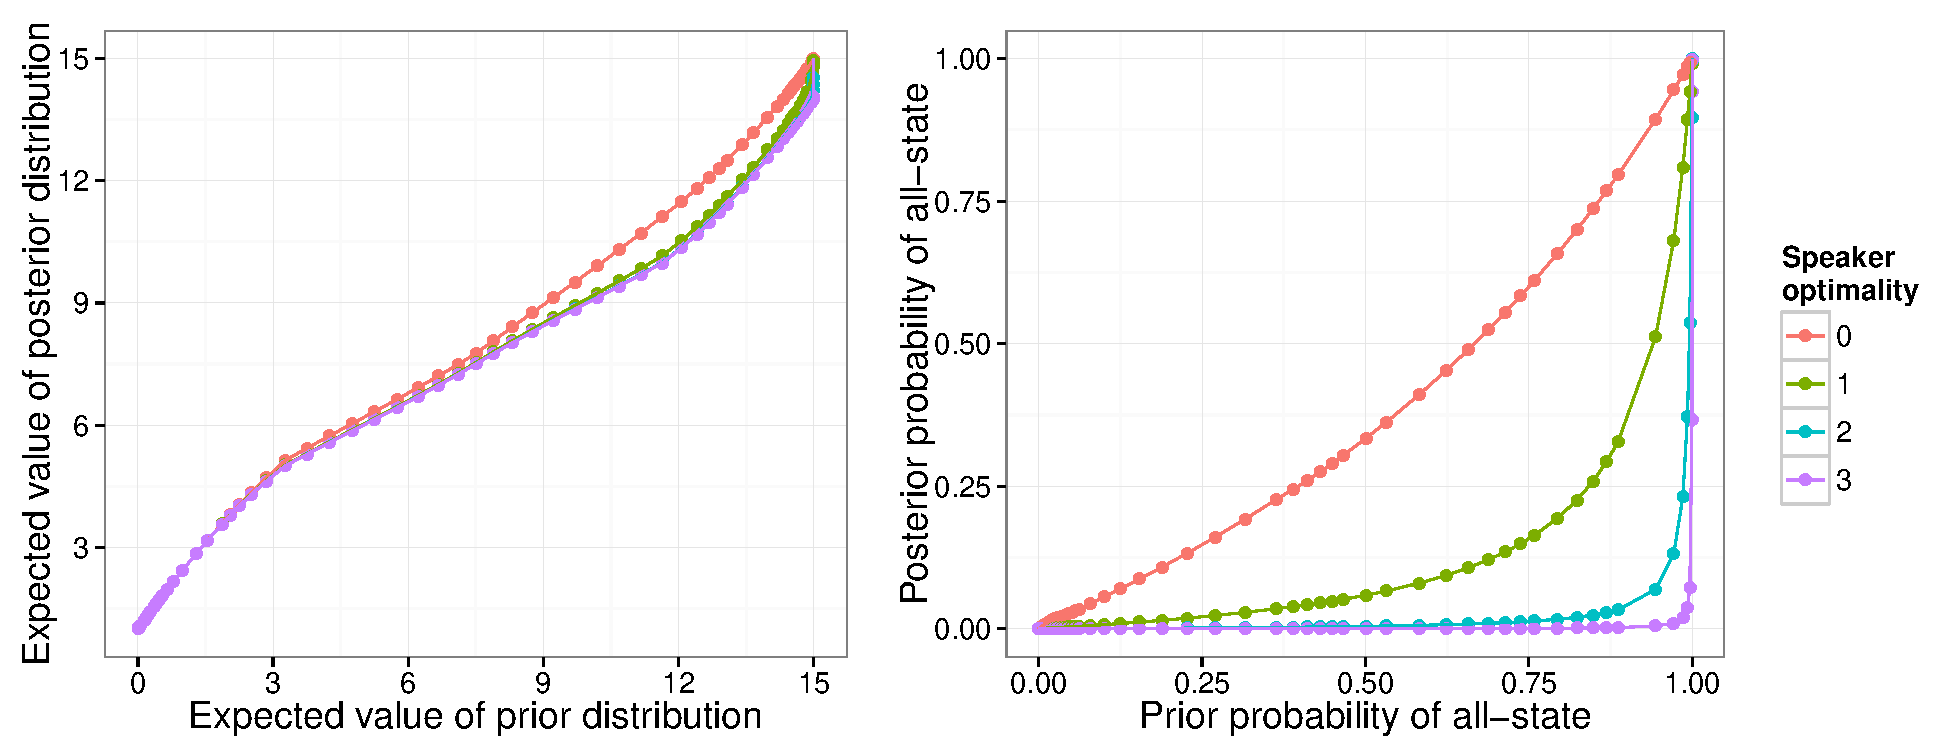
\includegraphics[width=\textwidth]{pics/beta-priordistributions}
%	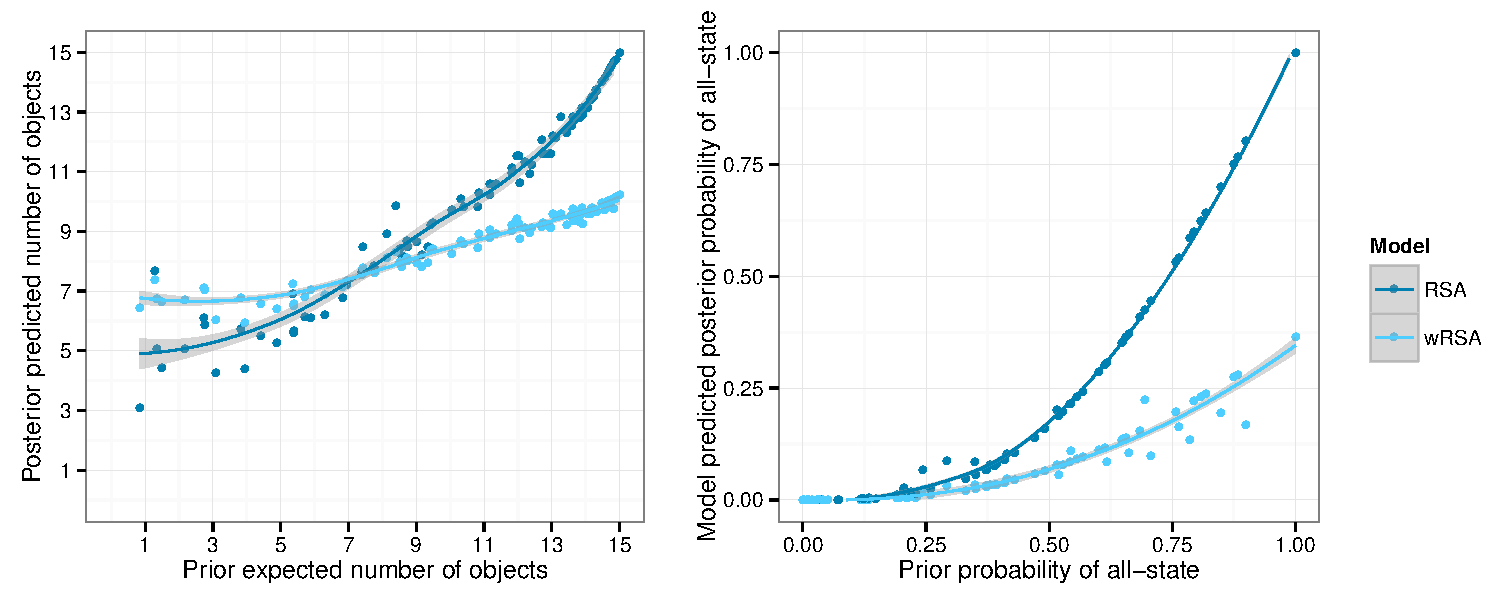
\includegraphics[width=\textwidth]{pics/rsa-predictions}
%	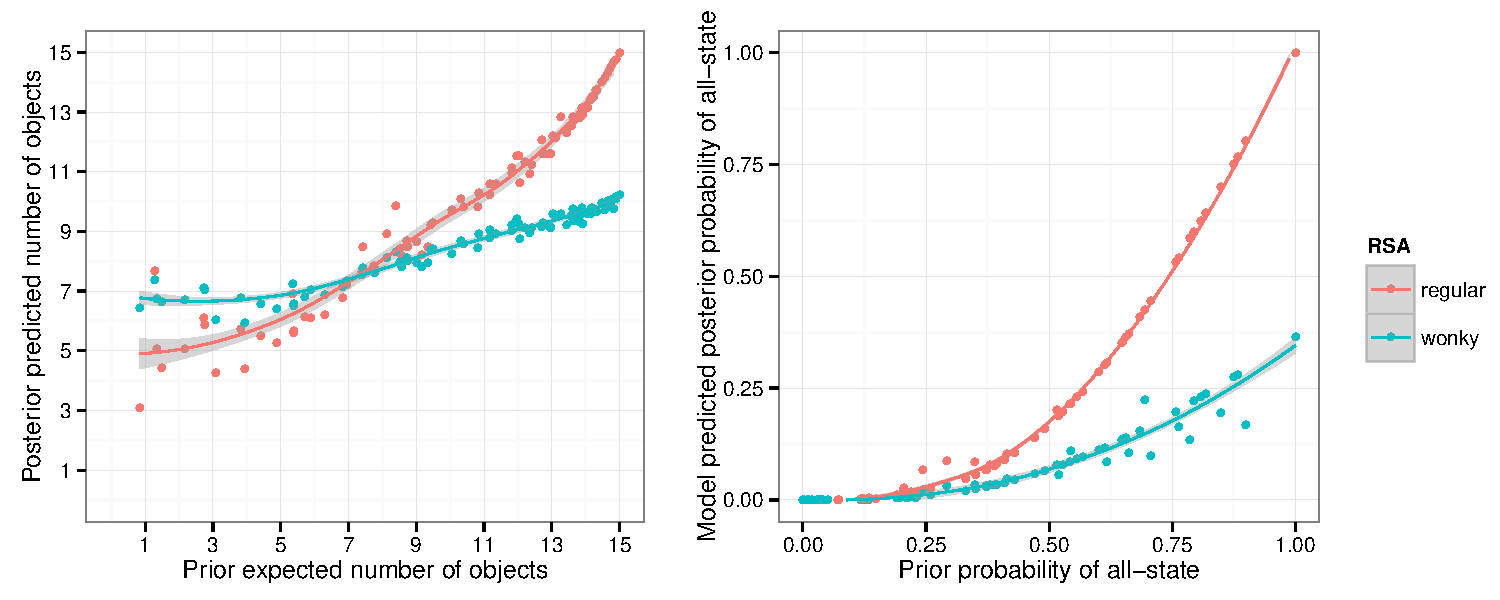
\includegraphics[width=\textwidth]{pics/rsa-predictions-uniform}	
%	\caption{For each item, RSA and wRSA model predicted $\mathbb{E}[P(s|u_{\textrm{some}})]$ as a function of $\mathbb{E}[P(s)]$ (left) and $P(s_{15}|u_{\textrm{some}})$ as a function of $P(s_{15})$ (right).\red{PLOT TO BE UPDATED WITH NEW BEST MODEL PREDICTIONS}
	\caption{\blue{RSA predictions for $\mathbb{E}[P(s|u_{\textrm{some}})]$ as a function of $\mathbb{E}[P(s)]$ (left) and $P(s_{15}|u_{\textrm{some}})$ as a function of $P(s_{15})$ (right) for different speaker optimalities $\lambda$.}
	\ndg{what is the line?}}
	\label{fig:rrsaexppredictions}	
\end{figure*}

In Figure \figref{fig:rrsaexppredictions} we show the predictions of RSA for \blue{hypothetical beta priors} \jd{i don't know how to talk about this; please modify as needed} in two different ways: the left panel shows the posterior expected number of affected objects as a function of the expected value of the prior belief distribution; the right panel shows the posterior probability of the state in which all objects are affected, as a function of the prior probability of that state, with speaker optimality parameters ranging from 0 (random speaker) to 3 for illustration. %\footnote{Here and below, model predictions are reported for parameter settings that were derived through \red{MH BRIEFLY DESCRIBE PROCEDURE}. Details of the procedure are provided in \appref{app:bayesianselection}.%That the individual model predictions look somewhat noisy is due to the different shapes of the prior distributions, such that for the same expected value of the distribution, the distribution itself can take different shapes, which are treated slightly differently by the model.}   %as $\theta$ varies. \red{put in figure showing the basic RSA predictions for allstate $P(s_{15}|u_{some})$ and expectation. this figure could also have wRSA predictions for later reference.} 
We see that the prior has a strong effect, which can be summarized by the two predictions described in the Introduction: 
\begin{enumerate}
	\item $P(s_{15}|u_{\textrm{some}}) \rightarrow 1$ as $P(s_{15})\rightarrow 1$\\That is, the posterior probability of the all-state after observing \emph{Some of the X Yed} approaches 1 as the prior probability of the all-state approaches 1.
	\item $\mathbb{E}[P(s|u_{\textrm{some}})] \simeq \mathbb{E}[P(s)]$ over the upper half of its range\\That is, the expected value of the posterior distribution after observing \emph{Some of the X Yed} tracks the expected value of the prior distribution.
\end{enumerate}

\blue{We next turn to an empirical test of these predictions by conducting two interpretation experiments, one each for each of the two predictions. Comparing model predictions to empirical interpretation data requires knowing listeners' prior beliefs. Rather than make these up (as we did for generating the predictions visualized in \figref{fig:rrsaexppredictions}) we measure them empirically. Thus, testing the two predictions proceeds in three steps: first, we collect empirical estimates of listeners' prior beliefs about a large number of domains. Second, we conduct two interpretation studies. Finally, we compare the model's predictions about interpretation probabilities (using the empirically elicited priors) to listeners' empirical interpretation data.} %, or rather, of the intuition that they may be incorrect.

%\section{Models of utterance interpretation}
%
%
%Recent Bayesian Rational Speech Act (RSA)  \cite{frank2012} and game-theoretic \cite{franke2011} models that treat communication as a signaling game \cite{lewis} between a speaker and a listener have successfully captured listeners' quantitative  behavior on a number of pragmatic inference tasks, including ad hoc Quantity implicature \red{ref}, M-implicature \red{ref}, scalar implicature \red{ref}, and embedded scalar implicatures \red{ref}. In these models, the listener reasons about likely utterances a speaker will produce who is trying to be informative with respect to a na\"ive listener. These models make clear predictions about how prior beliefs about states of the world should be integrated with listeners' expectations about utterances a speaker is likely to produce to communicate a particular state of the world. 
%
%\red{i think we should hold the math for the model section. it doesn't really add much here... without it, this section can be folded nicely into the introduction.}
%
%For concreteness, assume that $S = \{s_0, s_1, s_2, \dots, s_{15}\}$ is the set of states of the world, where the subscript indicates the number of objects (e.g., marbles) that exhibit a certain effect (e.g., sinking). Assume further that $U = \{u_{\textrm{all}}, u_{\textrm{none}}, u_{\textrm{some}}\}$, the set of utterances \emph{All/None/Some of the marbles sank}. The speaker chooses an utterance to convey $s$ proportional to the soft-max expected utility of producing $u$ to communicate $s$, where utility is determined by how uncertain a listener remains: \red{what's the expectation doing?}
%
%\begin{equation}
%P_{S_1}(u|s) \propto \mathrm{exp}({\lambda \mathbb{E} (\ln P_{\textrm{lex}}(s|u))})
%\end{equation}
%
%where $P_{\textrm{lex}}(s|u)$ is the literal interpretation probability resulting from each utterance's truth-functional meaning: $F_u: s \mapsto \{0,1\}$. \red{need to spell out lit listener since the prior enters there too} The listener's task is to infer a distribution over $S$, given an utterance $u$ produced by the above defined informative speaker. %$p(s|u)$, that is, the probability of the state of the world the speaker intended to communicate (e.g., how many friends came to a party), given that the speaker produced $u$ (e.g., \emph{some of my friends came to the party}). 
%By Bayes' rule: 
%\begin{equation}
%P_{L_1}(s|u)\propto P_{S_1}(u|s)\cdot P(s)
%\end{equation}
%That is, the inferred listener probabilities are proportional to the product of both the speaker's utterance probabilities and the listener's prior beliefs in different numbers of marbles sinking. Using a uniform prior over the state space, this model has been very successful at capturing \emph{scalar implicatures} \cite{grice1975}. These are inferences that arise in cases of utterances like \textit{Some of the marbles sank}, which typically give rise to the inference that not all of the marbles sank. Scalar implicatures fall out of the fact that the speaker probability of producing $u_{\textrm{some}}$ in $s_{15}$ is low (because there is an alternative utterance $u_{\textrm{all}}$ which has a higher probability of being used for $s_{15}$ because it is more informative about that state). However, the role of prior beliefs in RSA models remains under-explored, both with respect to scalar implicature computation as well as with respect to utterance interpretation more generally.
%
%
%%One important consequence of the standard RSA model is that the listener's prior beliefs will not affect the interpretation of $u$ very strongly, if at all,  where the semantics of $u$ is highly constraining, that is, where  $P_{\textrm{lex}}(s|u)$ is very peaked. For example, an utterance of \emph{All of the marbles sank} is highly constraining because all of the probability mass ends up on $s_{15}$ by virtue of the semantics of $u_{\textrm{all}}$ alone, regardless of how likely the listener believes marbles sink a priori.\footnote{We ignore hyperbolic interpretations of universal quantifiers here.} 
%
%One important consequence of the standard RSA model is that where the semantics of $u$ is weak---that is, where $F_u$ accepts many states---prior beliefs are predicted to have a large effect on the resulting listener belief distribution. For example, an utterance of \emph{Some of the marbles sank}, produced in a situation in which any of 0 - 15 of 15 contextually established marbles could have sunk, semantically only restricts the state space by one state (that in which 0 marbles sank). In this case, listeners' prior beliefs about sinking marbles will have a large effect on their posterior belief distribution. If the listener believes that marbles rarely sink, the utterance will be interpreted as conveying that fewer marbles sank than if the listener believes marbles almost always sink. The predictions this model makes for the interpretation of $u_{\textrm{some}}$ -- both for $P_{L_1}(s_{15}|u_{\textrm{some}})$ and for the expected value of $P_{L_1}(s|u_{\textrm{some}})$ as a function of $P(s_{15})$ and the expected value of $P(s)$, respectively  -- are shown in \figref{fig:rrsaexppredictions}. RSA predicts that the probability of the state in which all objects exhibit a certain effect increases with increasing $P(s_{15})$, such that for $P(s_{15})$ close to 1, $P_{L_1}(s_{15}|u_{\textrm{some}})$ approaches 1. Relatedly, with increasing expected value of the prior belief distribution $P(s)$, so is the expected value of the posterior belief distribution predicted to increase, approaching 1). \red{hmm... i think we either need to focus on the allstate probs for this motivation, or already point to the data from expt 1.}
%
%However, intuition is at odds with this prediction: for example,  \citeA{geurts2010} has observed that for events with very high prior probability of occurrence (e.g.~marbles sinking), observing an utterance of \emph{Some of the marbles sank} leads to very strong implicatures, that is, the subjective probability  that not all of the marbles sank is intuitively close to 0. Given the previous success of RSA models, this constitutes a striking puzzle, and one we set out to solve here. In doing so, we pursue the intuition raised at the very beginning of this paper: that sometimes, the speaker's utterance will lead the listener to infer that the world under discussion is wonky and she should therefore down-weight her prior beliefs in the computation of speaker meaning.
%
%
%Our contribution is two-fold: first, we collect empirical estimates of $P(s)$ and $P_{L_1}(s|u)$ to investigate the empirical effect of listeners' prior beliefs on interpretation. Second, we extend the RSA model to incorporate a free variable $\theta_{\textrm{wonky}}$ that captures the extent to which the listener believes the described event is wonky  and she should thus discount her prior beliefs when interpreting $u$. We refer to this model as \emph{wonky RSA (wRSA)} in contrast to \emph{regular RSA (rRSA)}. Wonkiness inferences in wRSA are triggered by the surprisal of a produced utterance $u$, given listeners' prior beliefs, capturing that listeners expect speakers' utterances to be both truthful and informative with respect to prior beliefs. To the extent that they are not, listeners will have to either infer that the speaker is being uncooperative, or else assume that they may need to revise their beliefs about the world. Here we pursue the latter possibility.
%
%This paper is structured as follows. We first report the results of three experiments (1, 2a, 2b) that show that while there is an effect of the prior on listeners' interpretations of sentences like \emph{Some of the marbles sank}, this effect is much smaller than predicted by rRSA. Exp.~3 provides evidence that listeners' beliefs about object or event wonkiness are indeed influenced by the surprisal of the utterance. Finally, we present wRSA as an extension of rRSA that incorporates the idea of backing off to alternate prior beliefs if the observed utterance suggests a wonky world. This model provides a much better fit to the empirical data from Exps.~2a and 2b than rRSA, and also provides a good fit to the wonkiness ratings obtained in Exp.~3.




\section{Experiment 1: prior elicitation} 
\label{sec:priors}

\ndg{it's kind of odd to me to put this section before the RSA description -- we don't know yet why we care about this prior... how about reversing the order, but breaking up the RSA section so that the basic model section shows schematic predictions with some standard priors (eg beta), and then the predictions with empirical priors are in the results to the priors section? this also makes the intro to priors less jarring: in contrast to the idealized priors just used we will use empirical priors so that no one ca accuse us of making them up...}\jd{order reversed and additional changes marked in blue. better?}

Obtaining good estimates of prior beliefs is crucial for testing any Bayesian model. Indeed, Bayesian approaches have recently been criticized for being lax in their treatment of priors \cite{jones2011, marcus2013}. To avoid this criticism, we empirically elicit estimates of prior beliefs. We measured listeners' prior beliefs about how many objects exhibit a certain effect (e.g., how many marbles sink) by following the four-step procedure described by \citeA{Speirs-Bridge2010}.

\subsection{Method}

\subsubsection{Participants}
We recruited 240 participants over Amazon's crowd-sourcing platform Mechanical Turk.\footnote{This experiment can be viewed at \url{http://cocolab.stanford.edu/cogsci2015/wonky/priors/sinking-marbles.html}.} Participants were paid \$0.50 for their participation. Here and in all other experiments reported in this paper, participants' IP address was limited to US addresses only and only participants with a past work approval rate of at least 95\% were accepted.

\subsubsection{Procedure and materials}

\jd{now one-step priors are reported, with four-step priors in footnote. replace broken link}

\blue{On each trial, participants read a one-sentence description of an event like \emph{John threw 15 marbles into a pool.} We were interested in obtaining estimates of a subsequent effect, in this case how many marbles participants believed sank. To this end, participants answered questions like \emph{How many of the marbles do you think sank?} by adjusting a slider that ranged from 0 to 15.} 

%Following the procedure in \citeA{Speirs-Bridge2010}, we elicited participants' beliefs in four steps:  first, they were asked to provide a lower bound on how many marbles sank. Then they were asked to provide an upper bound. Next, they were prompted for their best guess as to how many marbles sank. All three of these estimates were given by typing a number into a text field. Finally, they were asked to rate how confident they were that the interval they created captured the actual number of marbles that sank, by adjusting a slider with endpoints labeled ``not confident at all'' and ``very confident''. A full example of questions asked is provided in \eref{fourstep}.

%\eenumsentence{\label{fourstep}
%				\item \emph{Realistically, what do you think the lowest number of marbles that sank could be?}
%				\item \emph{Realistically, what do you think the highest number of marbles that sank could be?}
%				\item\label{bestguess} \emph{Realistically, what is your best guess at how many marbles sank?}
%				\item \emph{How confident are you that the interval you created, from lowest to highest, will capture the actual number of marbles that sank?}}
%

%We are most interested in participants' response to \eref{bestguess}, since, over the population, that will allow us to directly compute the prior probability of each number of marbles sinking. The questions always had the same forms as shown in \eref{fourstep}. 

\blue{Each item had a similar form: an initial sentence introduced 15 objects of a particular type (e.g., marbles) and was followed by a question. Each question had the form \emph{How many X do you think Yed?}, where \emph{X} was the head of the direct object noun phrase introduced in the first sentence (e.g., \emph{marbles}, \emph{cups}, \emph{balloons}) and \emph{Yed} was a verb phrase denoting an effect that the objects underwent (e.g., \emph{sank}, \emph{broke}, \emph{stuck to the wall}). Each verb phrase occurred with three different objects, e.g., \emph{sank} occurred with \emph{marbles}, \emph{cups}, and \emph{balloons}. Items were constructed to intuitively cover the range of probabilities as much as possible. Judgments were obtained for 90 items, of which each participant saw a random selection of 30 items.}\footnote{In a separate experiment with 120 participants, we replicated these priors in a four-step procedure described by \citeA[see also \appref{four-step-priors}]{Speirs-Bridge2010}. \red{Which priors were used as the basis for the analyses reported in the remainder of this paper did not affect the results; we therefore report only the results from the simple elicitation measure.}} 

\subsection{Results}

Each item received between 44 and 75 responses. Distributions of responses for each item were smoothed using nonparametric density estimation for ordinal categorical variables \cite{liracine2003} with the \verb|np| package in R \cite{hayfield2008}. For each item, we then computed its belief distribution's expected value and all-state probability. As intended, items covered a wide range of probabilities and expected values (see \figref{fig:probhist}). 

%Data from one participant, who provided a lower bound with a value greater than the upper bound on ten trials, were excluded. A further seven trials on which such reversals occurred were also excluded. This yielded an exclusion of 1\% of the data. Each item received between 10 and 30 ratings on each measure. We focus here on the best guess measure. Distributions of best guesses for each item were smoothed using nonparametric density estimation for ordinal categorical variables \cite{liracine2003} with the \verb|np| package in R \cite{hayfield2008}. For each item, we then computed its belief distribution's expected value and all-state probability. As intended, items covered a wide range of probabilities and expected values (see also \figref{fig:probhist}). 

\begin{figure}
\centering
%	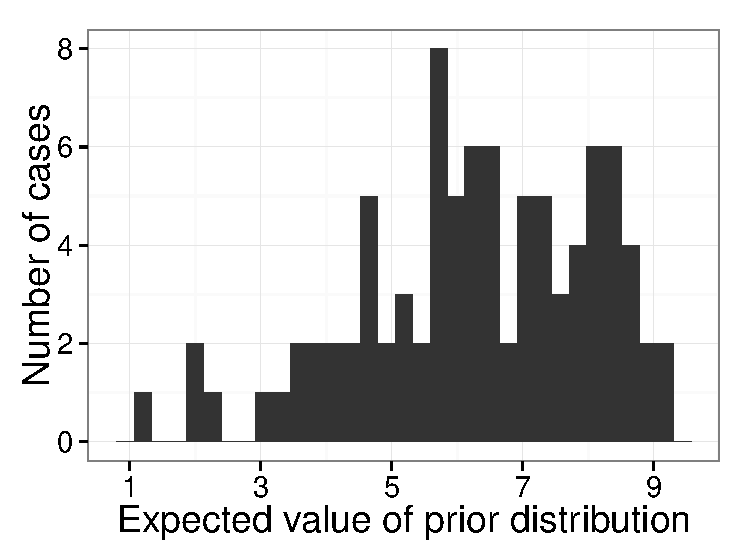
\includegraphics[width=.5\textwidth]{pics/priorexpectations-histogram}	
	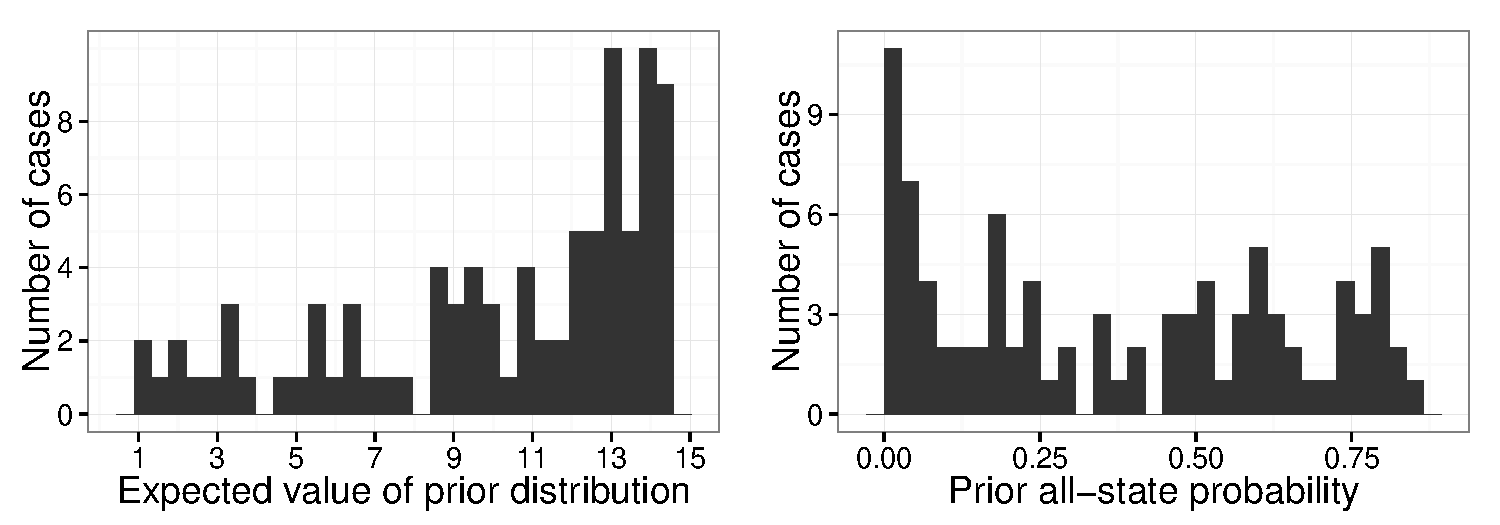
\includegraphics[width=\textwidth]{pics/priordistributions}	
	\caption{Histogram of expected values $\mathbb{E}[P(s)]$ of each empirically elicited and smoothed prior distribution (left) and histogram of prior probabilities $P(s_{15})$  of the all-state for each item (right).}
	\label{fig:probhist}	
\end{figure}

\blue{Next, we empirically measure participants' interpretation of utterances like \emph{Some of the marbles sank}. We use the priors elicited here to generate model predictions for interpretation, which we then compare to the results of the interpretation studies.}




\section{Experiment 2a and 2b: comprehension}  
\label{sec:comprehension}

Exps.~2a and 2b  measured participants' posterior beliefs $P(s|u)$ about how many objects exhibited a certain effect (e.g., how many marbles sank), after observing an utterance. The only difference between the experiments was the dependent measure. The dependent measures differed in order to directly and independently estimate the two values that the  predictions above are concerned with: $\mathbb{E}[P(s|u_{\textrm{some}})]$ and $P(s_{15}|u_{\textrm{some}})$, i.e., the expected number of X that are deemed to have Yed and the probability of all of the X having Yed (a measure of implicature strength), respectively, after observing the utterance \emph{Some of the X Yed}.

\subsection{Method}

\subsubsection{Participants}
We recruited 240 participants in each experiment (i.e., 480 total) over Amazon's Mechanical Turk. \blue{All participants had US American IP addresses and were self-reported native speakers of English.}\footnote{These experiments can be viewed at \url{http://cocolab.stanford.edu/cogsci2015/wonky/expectation/sinking-marbles.html} and \url{http://cocolab.stanford.edu/cogsci2015/wonky/stateprobs/sinking-marbles-nullutterance.html}}  Participants were paid \$0.70.
\ndg{should probably say something about how Ns were chosen, and particularly why 2b has twice as many Ss...}\jd{ran another 120 people in 2a, so N is now the same in both exps}

\subsubsection{Procedure and materials}

Participants read the same descriptions as in Exp.~1. They additionally saw an utterance produced by a knowledgeable speaker about the event, e.g.~\textit{John, who observed what happened, said: ``Some of the marbles sank''}. In Exp.~2a (just as in Exp.~1), they then provided a judgment of an effect, e.g.~\textit{How many of the marbles do you think sank?}, on a sliding scale from 0 to 15. In Exp.~2b they instead rated on sliding scales with endpoints labeled ``definitely not'' and ``definitely'', how likely they thought 0\%, 1-50\%, 51-99\%, or 100\% of the objects exhibited the effect.

Each participant saw 10 \emph{some} trials and 20 filler trials, of which 10 contained the quantifiers \emph{all} or \emph{none}, and the rest were utterances that did not address the number of objects that displayed the effect. These 10 additional fillers were intended to establish a baseline for participants' use of information about the prior. Of these, half were generic short fillers that were intended to communicate the prior, e.g., \emph{Typical}. The rest were longer sentences that addressed a different aspect of the described scenario, e.g.~\emph{What a stupid thing to do}.\footnote{See \appref{sec:items} for a complete list of items.} The utterances were randomly paired with 30 random items for each participant.

 
\begin{figure*}
	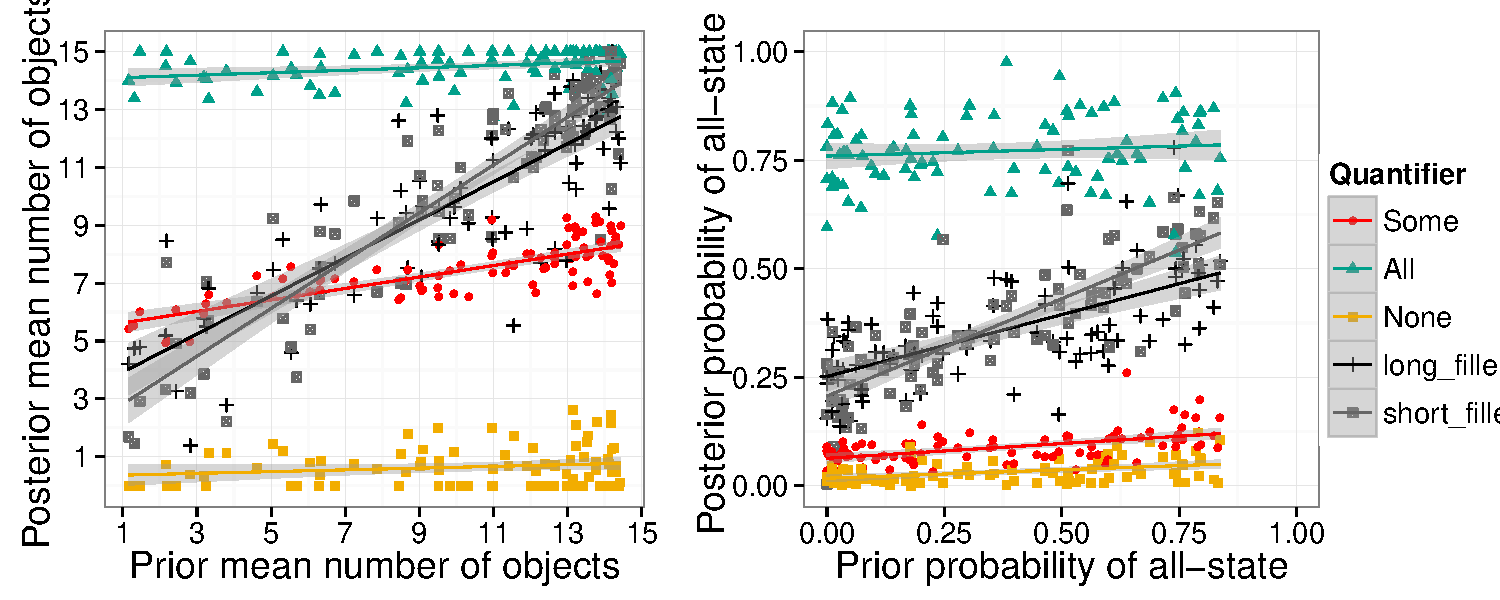
\includegraphics[width=\textwidth]{pics/empirical-results}	
	\caption{For each item and quantifier, empirical $\mathbb{E}[P(s|u_{\textrm{some}})]$ from Exp.~2a against $\mathbb{E}[P(s)]$ from Exp.~1 (left)  and empirical $P(s_{15}|u_{\textrm{some}})$ from Exp.~2b against  $P(s_{15})$ from Exp.~1 (right). \blue{Lines and gray ribbons indicate best loess fit through means and 95\% confidence intervals using a t-based approximation.}}
	\label{fig:empiricalresults}	
\end{figure*}

 
 \subsection{Results and discussion}

Data from Exp.~2a were analyzed without additional transformation. Slider ratings obtained in Exp.~2b were first subjected to normalization on a by-trial and by-participant basis, such that on each trial, a participant's ratings added to 1, i.e., constituted a proper probability distribution.%After normalization, data from eight participants in Exp.~2b were excluded from the analysis because these participants assigned less than 0.8 probability to the interpretation corresponding to the correct literal interpretation on literal \emph{all} and \emph{none} trials.
\footnote{In general, this task yielded noisier results than the task in Exp.~2a (as can be seen in the average lower probability of the all- state after observing \emph{all}, in the right panel of \figref{fig:empiricalresults}) because participants used the sliders in different ways. For example, for cases where  the all-state was true, some participants assigned non-zero probability to only the all-state, while others also always assigned some probability to the 51-99\% state.}

The main question of interest was whether the predictions of the basic RSA model laid out in the previous section were borne out in participants' judgments of how many X Yed after hearing an utterance with \emph{some}. Mean empirical $\mathbb{E}[P(s|u)]$ (expected value of the posterior distribution) and $P(s_{15}|u)$ (posterior all-state probability) are shown in \figref{fig:empiricalresults} for each item. Visual inspection of the graphs shows that the interpretation of utterances with \emph{all} and \emph{none} seems to be relatively unaffected by the prior, while the interpretation of \emph{some} displays a small effect. In comparison, participants strongly drew on their prior beliefs on filler trials, as evidenced in the much steeper slope of the filler trial best linear fit lines (the by-item correlation between empirical means and expected values of the prior was very high,  Pearson  $r$ = .93). 

To test whether the visual effect of the prior on the interpretation of \emph{some} is real, we conducted linear mixed effects regressions on the \emph{some} data from each experiment. For Exp.~2a, the number of X that Yed  was regressed onto a fixed effect of each item's prior expectation. For Exp.~2b, the  all-state probability was regressed onto a fixed effect of each item's prior all-state probability. The models also contained by-item and by-participant intercepts as well as by-participant slopes for the prior predictor.
%
For utterances of \emph{Some of the X Yed}, the mean number of objects judged to exhibit the effect increased with increasing expectation of the prior distribution ($\beta$=.19, $SE$=.02, $t$=10.10, $p$$<$.0001). Similarly, the probability of all 15 objects exhibiting the effect increased with increasing prior probability of doing so ($\beta$=.06, $SE$=.01, $t$=5.43, $p$$<$.0001). However, the size of these effects is, to say the least, much smaller than predicted by RSA.\footnote{Visually, the disparity between model predictions and empirical results can be seen by comparing the dark lines in \figref{fig:rrsaexppredictions} with the red lines in \figref{fig:empiricalresults}.}

One possible explanation for this highly attenuated effect of the prior is that participants simply did not bring world knowledge to bear on the interpretation of utterances. However, this possibility is ruled out by examining participants' performance in the filler conditions: in both Exps.~2a and 2b, the filler conditions closely tracked the prior (see \figref{fig:empiricalresults}). Additionally, that there is any effect of the prior at all suggests that participants are not entirely disregarding their prior beliefs.

Exps.~2a and 2b thus demonstrate that there is an effect of listeners' prior beliefs on the interpretation of utterances with \emph{some}. However, this effect is quantitatively much smaller than predicted by RSA, and qualitatively does not match the predictions identified above: the implicature is not canceled for extreme priors (contra prediction (1)) and the posterior expectation diverges from the prior expectation (contra prediction (2)).

\red{EXPAND MAKE SURE YOU HARP ON THE SPEAKER RELIABILITY ISSUE; BRING IN THE EXAMPLES FROM THE INTRO? In the next section, we account for this attenuated effect of the prior by extending the RSA model in a way that captures the intuition raised in the Introduction: when a speaker's utterance is too odd, a listener may decide that in order to uphold the assumption of speaker cooperativity, she should revise her initial beliefs about the domain that she presumed were in common ground. }


\section{Revising the common prior: `wonky RSA'}
\label{sec:wrsa}

To capture the idea that the pragmatic listener is unsure what background knowledge the speaker is bringing to the conversation, we extend the basic RSA model to capture uncertainty about an aspect of the language understanding setup itself---a technique that has been used recently for other aspects of pragmatic understanding \cite{goodmanlassiter,lassiter2013,bergengoodman2012,kao2014}. 
%corresponding to the choice of state prior. A lifted variable is a variable that the model (in particular, the pragmatic listener) reasons about explicitly instead of being given a value for it. 
In this case, we posit that the prior, now $P(s|w)$, depends on a ``wonkiness'' variable $w$, which determines whether to use the ``usual'' prior for this domain (empirically elicited in Exp.~1)  or a more generic back-off prior. We choose a uniform back-off prior, capturing that if the listener decides not to use the usual prior, she discards all beliefs about the domain and ascribes equal prior probability to each state:\footnote{\red{a footnote either briefly discussing other priors or delaying such a discussion to the general discussion}}
$$
P(s|w) \propto \begin{cases}
1  & \text{if } w\\
   P_{\text{usual}}(s) & \text{if not } w
  \end{cases}
  $$
 %
This prior is used in both the literal and pragmatic listeners, indicating that it is taken to be common ground. However, the $w$ variable is reasoned about only by the pragmatic listener---it is an inference the pragmatic listener makes about which assumptions are appropriate to the conversation (i.e.~which prior the speaker assumes). Using the notation of \sectionref{sec:rsa}:
\begin{eqnarray}
&&P_{L_0}(s|u,w)\propto \delta_{\denote{u}(s)} \cdot P(s|w)\\
&&P_{S_1}(u|s,w) \propto \mathrm{exp}({\lambda \ln P_{L_0}(s|u,w))}\\
&&P_{L_1}(s,w|u)\propto P_{S_1}(u|s,w)\cdot P(s|w) \cdot P(w)
\end{eqnarray}
We refer to this model as wRSA. Notice that the value of $w$ inferred by the listener will depend on $P_{S_1}(u|s,w)$: if a given utterance can't be explained by the usual prior, because it is unlikely to be uttered under any plausible world state $s$, then the pragmatic listener will infer that the world is wonky, and back off to the uniform prior.
That is, if the utterance is odd, the listener will revise her opinion about what world knowledge is appropriate to use to recohstruct the speaker's meaning. %\red{we need to explain where oddness comes from -- maybe there's an easy graphical way of showing how for items with different priors, a `some' utterance is more or less wonky, by showing the marginal probabilities of observing each utterance for these different items?}

\red{THIS WHOLE BIT NEEDS TO BE UPDATED IN RESPONSE TO MH'S NUMBERS To make predictions for Exps.~2 from wRSA we use the inferred priors from Exps.~1 as $P_{\text{usual}}(s)$ for each item. The wonkiness prior $P(w)$ and the speaker optimality parameter $\lambda$ are fit to optimize mean squared error (MSE) with Exp.~2 data. The optimal parameters ($\lambda = 2$, $P(w) = 0.5$) resulted in an MSE of 2.15 (compared to 14.53 for RSA) for the expected number of objects, and 0.01 (compared to 0.07 for RSA) for the all-state probability. The better fit of wRSA compared to RSA can be seen in the comparison of \figref{fig:rrsaexppredictions} and \figref{fig:empiricalresults}: in both cases, wRSA (light blue lines) predicts a much attenuated effect of the prior compared to regular RSA (dark blue lines), in line with the empirical data. Furthermore, wRSA does not make either of the problematic predictions identified earlier for regular RSA.}


These results are encouraging: wRSA is able to account for the qualitative and quantitative departures of participants' behavior from RSA, with respect to the effect of the prior. However, the skeptical reader may wonder whether the attenuated effect of the prior is really caused by listeners inferring that \emph{the world is wonky} when observing an odd utterance. Maybe listeners' disregard for the prior is instead triggered by an inference that \emph{the speaker is unreliable}. There are at least two ways to test whether a world wonkiness story or a speaker reliability story is more plausible. One is to generate model predictions for wonkiness probability and compare them to empirical wonkiness estimates. Another is to lesion the model to simulate different ways in which speakers could be unreliable, and compare the resulting model predictions to empirical data from an experiment that manipulates speaker reliability. The next two sections report the results of conducting each of these tests.

\section{Experiment 3: wonkiness}
\label{sec:wonkiness}

The wRSA model makes predictions about the probability that a given world is wonky (i.e.~is governed by an abnormal prior) after observing an utterance; see the left panel of \figref{fig:wonkymodel} for predicted wonkiness probabilities for $u_{\textrm{all}}$, $u_{\textrm{none}}$, and $u_{\textrm{some}}$ \red{using the  optimal $P(w)$ and $\lambda$ parameters from fitting wRSA to the Exp.~2 data UPDATE ONCE MH'S NUMBERS ARE IN}.
Note the U-shaped curve, in which the world is judged wonky if $u_{\textrm{some}}$ is used in worlds with extreme priors. Exp.~3 tested these predictions by asking participants whether they believed the described situation was normal for each utterance and item from Exps.~2a and 2b.

\begin{figure}
\centering
%	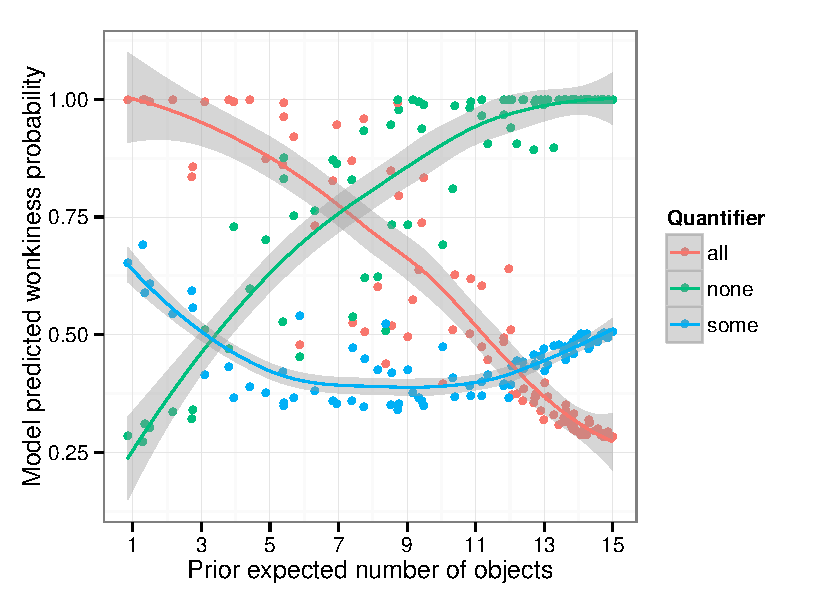
\includegraphics[width=.5\textwidth]{pics/model-wonkiness-binomial}
%	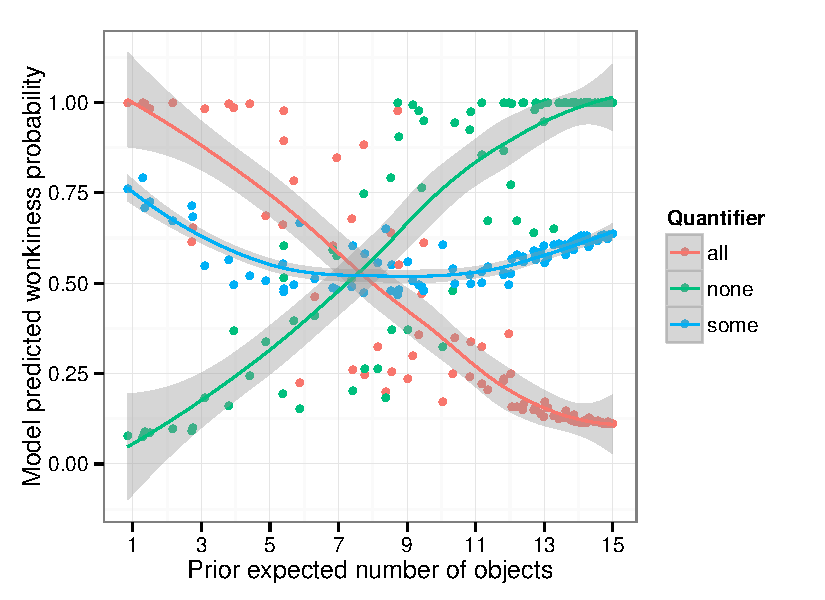
\includegraphics[width=.5\textwidth]{pics/model-wonkiness-uniform}
%	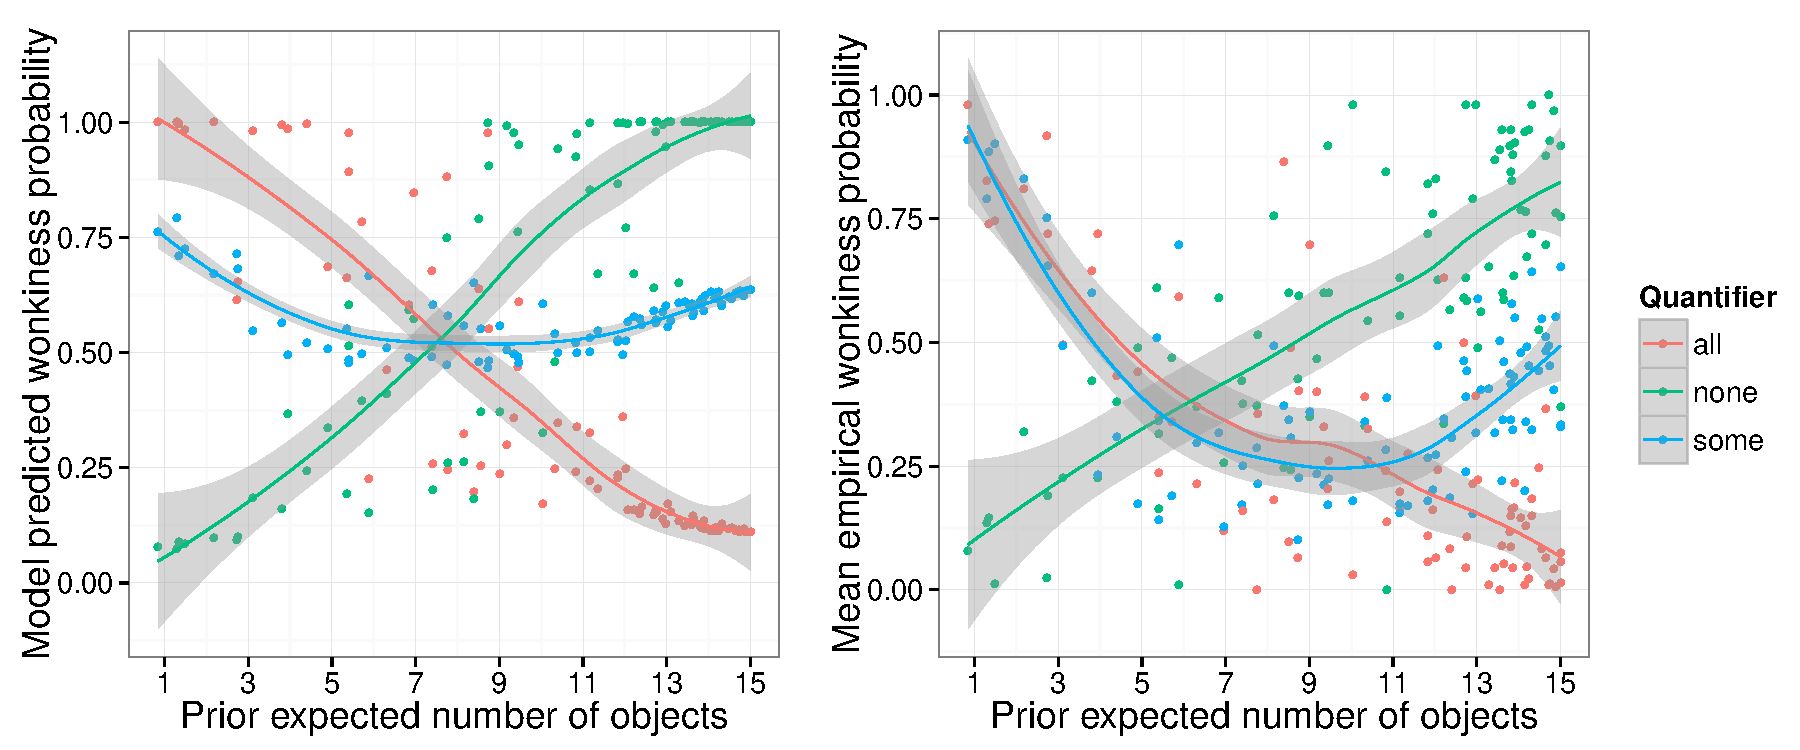
\includegraphics[width=.9\textwidth]{pics/wonkiness-fullplot}
	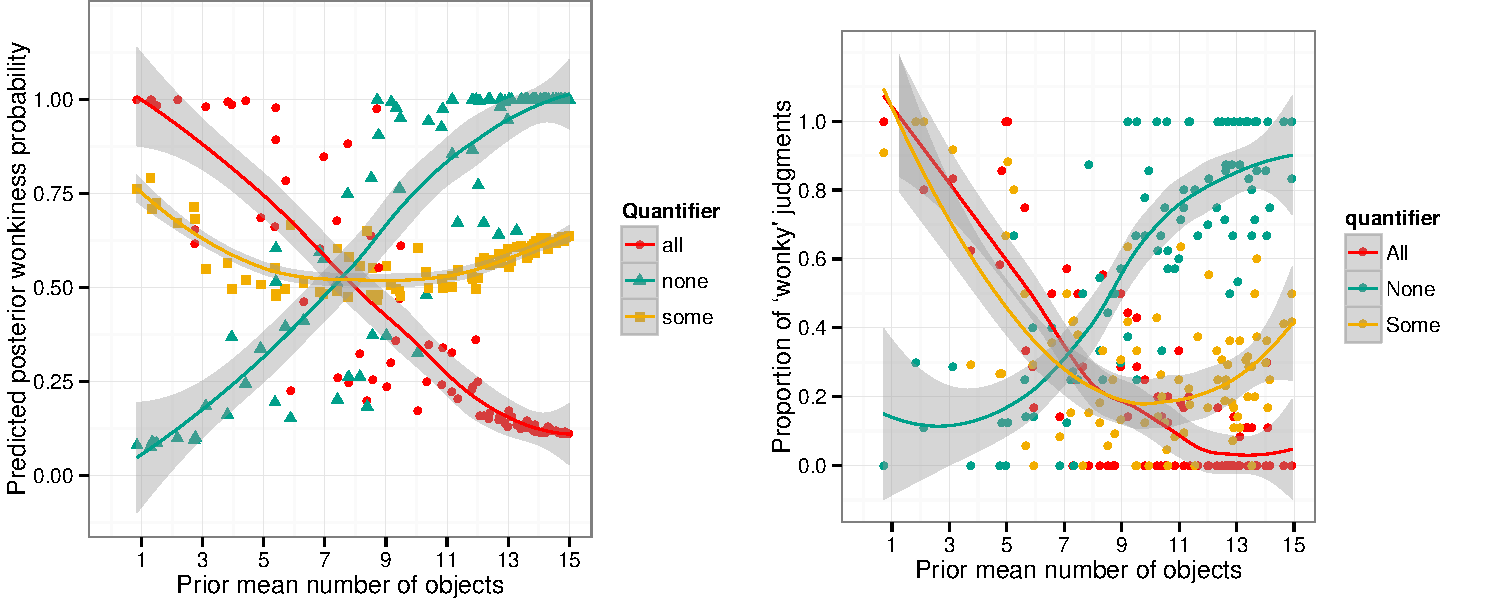
\includegraphics[width=.9\textwidth]{pics/wonkiness-results}
	\caption{For each item, predicted (left) and empirical (right) wonkiness probability after observing an utterance ($u_{\textrm{all}}, u_{\textrm{none}}, u_{\textrm{some}}$), as a function of the prior expected number of affected objects. \red{UPDATE THIS PLOT WHEN MH IS DONE}}
	\label{fig:wonkymodel}	
\end{figure}

\subsection{Methods}

\subsubsection{Participants}
We recruited 120 participants over Amazon's crowd-sourcing platform Mechanical Turk.\footnote{This experiment can be viewed at \url{http://cocolab.stanford.edu/cogsci2015/wonky/wonkiness/sinking-marbles-normal.html} \jd{change the experiment that the link points to (currently pointing at slider experiment)}} Participants were paid \$0.50.

\subsubsection{Procedure and materials}

The procedure and materials were identical to those of Exps.~2a and 2b, with the exception of the dependent measure. Rather than providing estimates of how many X they believed Yed, participants were asked  whether they thought that the objects involved in the scenario were normal objects, for example \emph{Do you think these are normal marbles?}  They responded by checking a ``Yes'' or ``No'' radio button.\footnote{The results replicate qualitatively using at least two different dependent measures: in one study, instead of being asked about the objects involved in the event, participants were asked about the normalcy of the event directly. In a different study, instead of performing a binary forced choice task, they were asked to indicate how likely it was that the objects  involved in the scenario were normal objects, by adjusting a slider with endpoints labeled ``definitely not normal'' to ``definitely normal.'' \jd{Results in Appendix? Supplementary materials?}}

\subsection{Results and discussion}

%The extreme ends of the sliders were coded as 1 (``definitely not normal'', i.e., wonky) and 0 (``definitely normal'', i.e., not wonky). We interpret the slider values as probability of world wonkiness. Mean wonkiness probability 

Proportion of ``No'' (not normal, i.e., wonky) choices are shown in the right panel of \figref{fig:wonkymodel} and qualitatively mimic wRSA's predictions (see left panel of \figref{fig:wonkymodel}). For $u_{\textrm{all}}$ and $u_{\textrm{none}}$, increasing the prior expectation of Xs Ying resulted in a linear decrease and increase in the probability of wonkiness, respectively. For $u_{\textrm{some}}$, the pattern is somewhat more intricate: probability of wonkiness initially decreases sharply, but rises again in the upper range of the prior expected value. 
%
%\begin{figure}
%	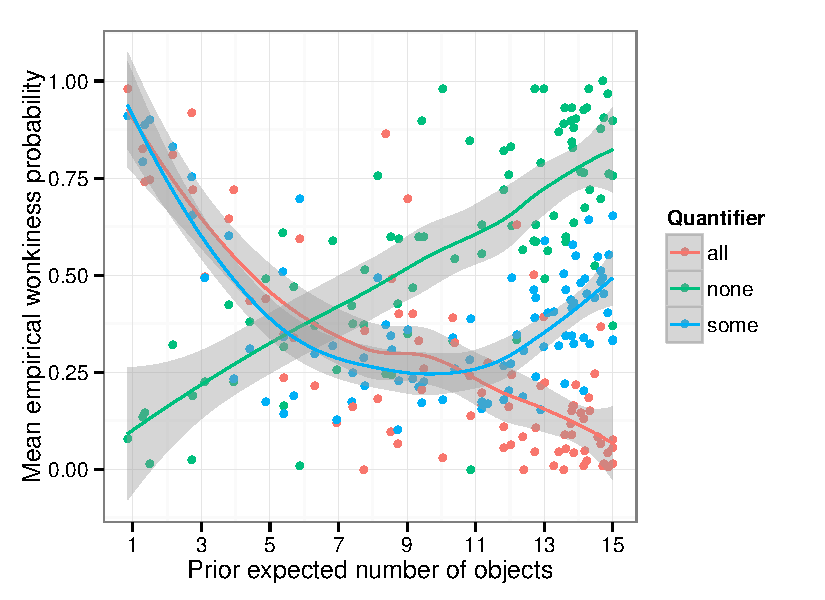
\includegraphics[width=.5\textwidth]{pics/empirical-wonkiness}
%	\caption{For each item, mean empirical wonkiness probability after observing an utterance ($u_{\textrm{all}}, u_{\textrm{none}}, u_{\textrm{some}}$), as a function of the prior expected  number of affected objects.}
%	\label{fig:wonkyratings}	
%\end{figure}

Qualitatively, the model captures both the linear increase and decrease in wonkiness probability for $u_{\textrm{all}}$ and $u_{\textrm{none}}$, respectively. Importantly, it also captures the asymmetric U-shaped wonkiness probability curve displayed by $u_{\textrm{some}}$. Intuitively, this shape can be explained as follows: for very low probability events, it is surprising to learn that such an event took place (which is what is communicated by $u_{\textrm{some}}$), so wonkiness is high. For medium probability events, learning that this event took place is not very surprising, so wonkiness is relatively low. For high probability events, $u_{\textrm{some}}$ may be literally true, but it is not useful in the sense of providing the listener new information, hence it is again surprising. For comparison to the comprehension data fit, \red{the model's MSE for empirical wonkiness probability predictions, using the best parameters from fitting the model to the comprehension data, was 0.07 UPDATE IN RESPONSE TO MH'S NUMBERS}. 

That the wonkiness probability predictions are borne out in the empirical data provide further support for wRSA, and for the idea that listeners revise their prior beliefs online when encountering an odd utterance. %\red{put in here somewhere the relation between wonkiness and the comprehension data: for all and none, while there are huge changes in wonkiness by prior, we don't expect this to show up in the comprehension data because the semantics of the utterances restricts the interpretation to just one state, regardless of the prior. but for "some", which has a weak semantics, wonkiness shifts the overall interpretation in a way that compresses the effect of the prior}
\ndg{we should say something more directly about how the empirical wonkiness judgements being much stronger than the model predictions...}

\section{Exp.~4: speaker reliability}
\label{sec:speakerreliability}

\ndg{i moved the section break here and massaged this section intro a lot. look it over...}

The skeptical reader may still not be convinced that what is driving the attenuated effect of the prior is that listeners revise their beliefs about the world (or about the event, or the objects involved in the event---we return to this distinction in the general discussion). A prima facie alternative possibility, raised at the end of \sectionref{sec:wrsa}, for why prior beliefs have a much smaller effect than expected on utterance interpretation, is that listeners believe that the speaker is an unreliable or uncooperative speaker (recall this paper's opening examples). For example, maybe participants in the studies reported thus far believed that the speaker was a) lying, b) not trying to be informative, or c) not knowledgeable about the precise state of the world, i.e., about how many X Yed, despite having been told so.
Yet participants were happy to interpret the speaker's utterances literally in the \emph{all} and \emph{none} conditions, suggesting they didn't believe the speaker was simply lying. 
Further, the wonkiness judgments obtained in Exp.~3 qualitatively match the wRSA model's predictions, which relies on speaker reliability and cooperativity, suggesting that participants didn't take the speaker to be ignorant or malingering.
  
However, there is an even clearer reason to doubt speaker reliability explanations for the observed attenuated effect of the prior: if the speaker was  unreliable, intuition and the (RSA and wRSA) model predict that listeners should use their prior world knowledge  \emph{more} strongly, not less than if the speaker was reliable. This is simply because an unreliable speaker provides less new information to a listener, and thus changes the listener's beliefs less from her prior.
%%ndg: this example is probably interpreted more strongly, as understatement not unreliability.
%For example, if my very successful but understated friend says that he did ``OK'' on a job interview, I'll be more likely to disregard his pronouncement of mediocre performance and expect him to have done very well. 
For instance, recall our opening example: if Mary knows that John often says wild things to make fun of her gullibility, she may explain away his utterance of \emph{All of the baseballs stuck to the wall} as a lie, and stick to her prior belief that baseballs do not stick to walls.  
%That is, speaker unreliability (well intentioned or not), if so perceived by listeners, intuitively leads listeners to much more strongly rely on their prior beliefs and discount the speaker's utterance.

%From the model's perspective, we can think about speaker unreliability in terms of different ways of lesioning the model. 
There are different ways to modify the model to capture an unreliable speaker.
Recall that the speaker chooses utterances in proportion to the informativeness of that utterance to a literal listener. One way to `lesion' the model is thus to let the speaker produce a random true utterance (as opposed to an informative true utterance). Another way is to let the speaker produce an utterance at random from the set of alternatives, regardless of whether it is true. These changes affect the pragmatic listener's likelihood function, hence resulting in different interpretation probabilities. In particular, the truthful but uninformative speaker somewhat increases the effect of the prior on the posterior all-state probability in wRSA, and the neither truthful nor informative speaker further increases that effect (as intuition suggests). These model predictions are shown for the items used in Exps.~1-3  in \figref{fig:speakerreliability-model}, \red{using the best parameters ($\lambda$ = 2, $P(w)$ = .5) from the model fitting reported in \sectionref{sec:wrsa}. UPDATE THIS AND THE PREDICTION PLOT ONCE MH IS DONE}

\begin{figure}
	\centering
	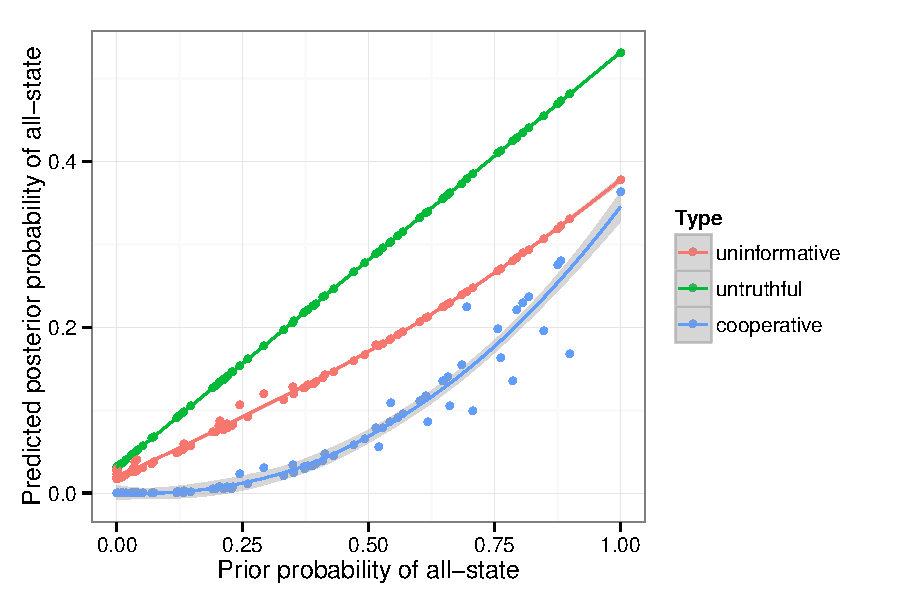
\includegraphics[width=.6\textwidth]{pics/modelpredictions-unreliablespeaker}
	\caption{For each item, predicted mean posterior all-state probability against  prior all-state probability, for uninformative, untruthful, and cooperative speakers. (Note that the cooperative speaker predictions are repeated from \figref{fig:rrsaexppredictions}). \red{UPDATE THIS PLOT ONCE MH IS DONE}}
	\label{fig:speakerreliability-model}	
\end{figure}

These considerations make the following prediction: if speaker reliability is explicitly manipulated, listeners' interpretations of \emph{Some of the X Yed} should be much more strongly governed by their prior beliefs when the speaker is unreliable (either untruthful or uninformative) than when the speaker is reliable/cooperative. That is, we expect a replication of Exp.~2b for reliable, but not unreliable speakers.\footnote{Indeed, the unreliable speaker conditions can be seen as a \emph{positive control} in the sense that they are predicted to show a strong effect of the prior in the situations where we have found an attenuated effect in our key experimental conditions.}
If, instead, there is something more fundamentally wrong with RSA models and the attenuated effect of the prior on comprehension is driven by listeners' perception of the speaker as unreliable, further decreasing speaker reliability should have no effect on how strongly the prior influences listeners' interpretations. If anything, explicitly unreliable speakers should further diminish the effect of the prior. %We test the prediction about speaker reliability in Exp.~4.

Exp.~4 explores how speaker reliability interacts with prior beliefs in the interpretation of the same utterances used in Exps.~1-3. %As discussed in the previous section, the wRSA model predicts that listeners' interpretation of \emph{Some of the X Yed} should be more strongly affected by their prior beliefs (as elicited empirically in Exp.~1) when the speaker is perceived as unreliable than when the speaker is perceived as reliable. 
There are different ways in which speaker reliability can be construed. 
Parallel to the two model `lesions' just described, we would like to manipulate speaker reliability in such a way as to lead listeners to expect underinformative or untruthful reports of  events. 
To this end, we introduce two unreliable speakers: a speaker who has an incentive to be misleading in a courtroom scenario and a drunken speaker. \ndg{at some point cite bonnefon's work on drunken SI?}\jd{i wrote to him and it appears that sadly, the results didn't replicate.} These speakers are contrasted within participants with a reliable speaker.

\subsection{Method}

Exp.~4 was very similar to Exp.~2b in method, but used only half of the items and a blocked design. In each block, the speaker who observed and subsequently described events remained the same throughout the block. The speaker's reliability was established via a short cover story at the beginning of each block. This allowed us to compare the effect of prior beliefs on participants' interpretations of \emph{Some of the X Yed} uttered by speakers of differing reliability.

\subsubsection{Participants}

We recruited 120 participants over Amazon's Mechanical Turk.\footnote{This experiment can be viewed at \url{http://cocolab.stanford.edu/cogsci2015/wonky/speakerreliability/sinking-marbles.html}.} Participants were paid \$1.00 for their participation. 

\subsubsection{Procedure and materials}

Participants were first introduced to a party scenario with three (randomly generated) characters, here James, Emily, and Robert:

\begin{quote}
Yesterday, James, Emily, and Robert went to a big, crazy party that lasted all day. Everyone was playing games and having fun. In this study, you'll read about James, Emily, and Robert's experiences at the party and answer simple questions.
\end{quote}

They then proceeded through three blocks of fifteen trials each, for a total of 45 trials. On each block, one of the three characters introduced initially was the speaker. Speaker reliability was manipulated via a short description of the speaker at the beginning of each block. One speaker was reliable (\emph{sober} condition) and two were unreliable (\emph{drunk} and \emph{court} condition). Block order was randomized.  The following are examples of speaker descriptions for the block order \emph{sober - drunk - court}.

\emph{Sober:}
\begin{quote}
Flashback to the party: James likes to comment on events he observes. He also likes to keep a clear mind, so he is staying sober. He's having a great time going around observing what people are doing and commenting on what happens.
\end{quote}

\emph{Drunk:}
\begin{quote}
Now you know how James experienced the party. Next up is Emily.

Flashback to the party: Emily is pretty drunk. Her speech is slurred. At one point she thinks she sees a flying pig. But she's having a great time going around observing what people are doing. She describes what happens to anyone who will listen.
\end{quote}

\emph{Court:}
\begin{quote}
Now you know how Emily experienced the party, too. Next up is Robert.

It's the day after the party. Robert has been asked to appear in court. He was witness to events at the party that resulted in damaged property. The prosecutor asks him questions about the events that transpired. In each case, John saw exactly what happened. But he also wants to protect his friends.
\end{quote}

\begin{table}
\caption{Overview of trial structure in the different blocks (\emph{sober, drunk, court}) of Exp.~4.}
\begin{tabular}{l p{4.2cm} p{4.2cm} p{4.2cm}}
\toprule
 & \centering \emph{sober} & \centering \emph{drunk} & \centering \emph{court} \tabularnewline
\midrule
Event & \multicolumn{2}{c}{At the party, Diane threw 15 marbles into the pool.} & The prosecutor says: ``Diane threw 15 marbles into the pool. What happened next?''\\
\midrule
Speaker & James, who interestedly observed what happened, says, & Emily, who drunkenly observed what happened, says, & Robert, who observed what happened but wants to protect his friends, says,\\
\midrule
Utterance & \multicolumn{3}{c}{``Some of the marbles sank.''}\\
\midrule
Question & \multicolumn{3}{c}{How many marbles sank?}\\
\bottomrule
\end{tabular}
\label{tab:trialstructure}
\end{table}

On each trial, participants performed the same task as in Exp.~2b: they saw a sentence introducing an event (e.g., \emph{At the party, Diane threw 15 marbles into the pool}), followed by a sentence about the speaker (e.g., \emph{James, who interestedly observed what happened, says,}), followed by the speaker's utterance (e.g., \emph{``Some of the marbles sank''}). They were then asked to rate on four sliding scales with endpoints labeled ``definitely not'' and ``definitely'', how likely they thought 0\%, 1-50\%, 51-99\%, or 100\% of the objects (e.g., marbles) exhibited the effect (e.g., sank). The different speaker scenarios made it impossible to maintain an identical trial structure across blocks, but we attempted to minimize differences. See \tableref{tab:trialstructure} for an overview of trial structure in each block.

In Exp.~4, only half of the items from Exps.~1-3 were used; those 45 that described events that could plausibly have occurred at a day-long party, while nevertheless spanning the entire range of prior probabilities. See \appref{sec:items} for the full list of items; the first half of items were used in Exp.~4. Each block contained the same distribution of utterances: two \emph{all} trials, two \emph{none} trials, two short filler trials, two long filler trials, and seven \emph{some} trials. Items were distributed over utterances so that each participant saw each item once, i.e., no participant saw for example the \emph{sinking marbles} item with both the \emph{some} and the \emph{all} utterance.

\subsection{Results and discussion}

\begin{figure}
	\centering
	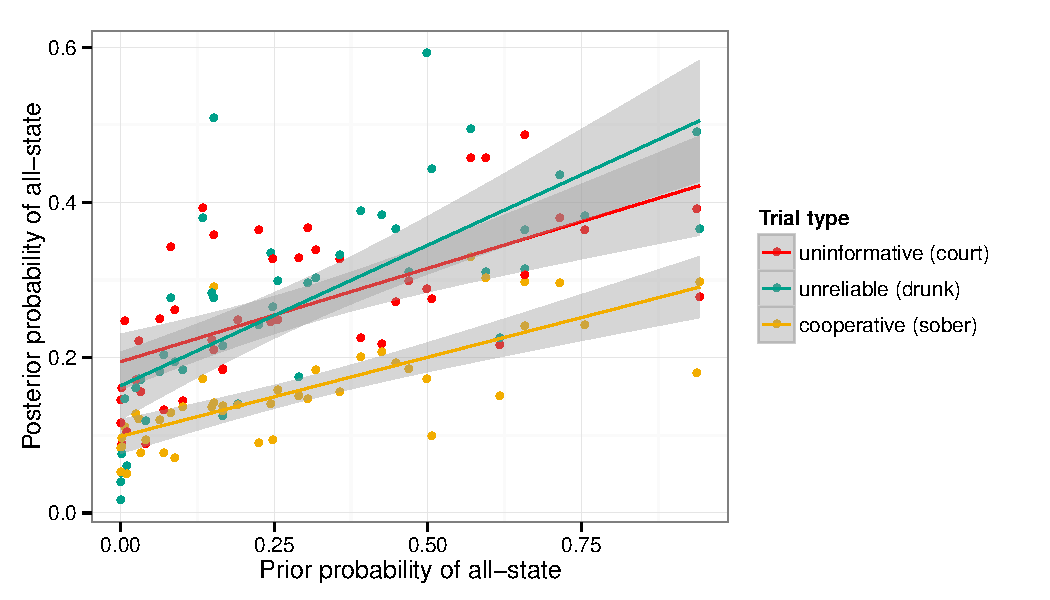
\includegraphics[width=.6\textwidth]{pics/speakerreliabilityresults}
	\caption{For each item, empirical mean posterior $P(s_{15}|u_{\textrm{some}})$ against  prior $P(s_{15})$ from Exp.~1, separately for reliable (\emph{sober}) and unreliable (\emph{drunk, court}) speakers.}
	\label{fig:speakerreliability}	
\end{figure}

Mean all-state probability ratings after observing  the \emph{some} utterance in the different speaker reliability conditions are shown in \figref{fig:speakerreliability}. While the reliable (\emph{sober}) speaker condition tracks the results from Exp.~2b very closely, the unreliable speaker conditions (\emph{court, drunk}) display a much greater effect of prior beliefs on the posterior probability of the all-state. This is borne out in a linear mixed effects regression model predicting the posterior all-state probability from fixed effects of prior all-state probability, speaker reliability, trial number (to account for adaptation over the course of the experiment), and their interactions. Speaker reliability was coded as a binary variable (reliable vs.~unreliable) and centered. \red{I coded it this way because so far I hadn't really been thinking about trying to tease apart the uninformative vs.~untruthful speaker. Don't know if it's worth pursuing the difference between the two. We could also just leave out Figure 5 and describe the pattern.} 
\ndg{i think it's worth also reporting a version of the regression that separates the two unreliable conditions. maybe as a binary predictor for unreliable and another for untruthful? if the untruthful coefficient is reliable it's cool, and if not we say this effect is either absent or too small to observe in current setup.}\jd{should we also include literal ocnditions? in that case we need more data.}
The all-state probability and trial number predictors were likewise centered before entering the analysis. The model included by-participant and by-item random intercepts and slopes for all fixed effects. 

%                                          Estimate Std. Error t value
%(Intercept)                               0.250349   0.012666  19.765
%cAllPriorProbability                      0.292455   0.048281   6.057
%cReliability                              0.126185   0.014972   8.428
%cTrial                                    0.003198   0.000354   9.034
%cAllPriorProbability:cReliability         0.151732   0.049249   3.081
%cAllPriorProbability:cTrial               0.004016   0.001246   3.223
%cReliability:cTrial                       0.000423   0.000900   0.470
%cAllPriorProbability:cReliability:cTrial -0.001125   0.002662  -0.423

There was a main effect of prior all-state probability such that the posterior all-state probability increased with increasing prior all-state probability ($\beta$=.30, $SE$=.05, $t$=6.1, $p$$<$.0001). There was also a main effect of speaker reliability, such that posterior all-state probability was judged higher when the speaker was unreliable ($\beta$=.13, $SE$=.01, $t$=8.4, $p$$<$.0001). In addition, there was an interaction between prior all-state probability and speaker reliability such that the slope of the prior all-state probability effect was shallower for the reliable speaker than for the unreliable speakers ($\beta$=.15, $SE$=.05, $t$=3.1, $p$$<$.01). Finally, we also observed adaptation effects: there was a main effect of trial such that all-state probability was rated as greater as the experiment progressed ($\beta$=.003, $SE$=.0003, $t$=9.0, $p$$<$.0001). We also observed an interaction of prior all-state probability and trial number, such that the prior had a greater effect on interpretation later in the experiment ($\beta$=.004, $SE$=.001, $t$=3.22, $p$$<$.01). \jd{shall i get rid of this last bit of analysis alltogether? i already deleted the figure and the description of the interaction in response to your comment.} %This is visualized in \figref{fig:speakerreliability-byblock}: while there is no change in how utterances of unreliable speakers are treated, reliable speakers are treated as more and more unreliable as the experiment progresses. This is interesting because it suggests that listeners are drawing a higher-level inference about speakers being unreliable in this context (where the context may be this particular party, or  this particular experiment), such that participants who had evidence that there were unreliable speakers in this scenario also took the sober speaker less seriously.\footnote{Note that in principle the reverse could have happened, that is, evidence for the presence of reliable speakers could have resulted in treatment of the unreliable speakers as more reliable over time. We see no evidence for this.} \ndg{i don't thin we need this fig.}
%
%\begin{figure}
%	\centering
%	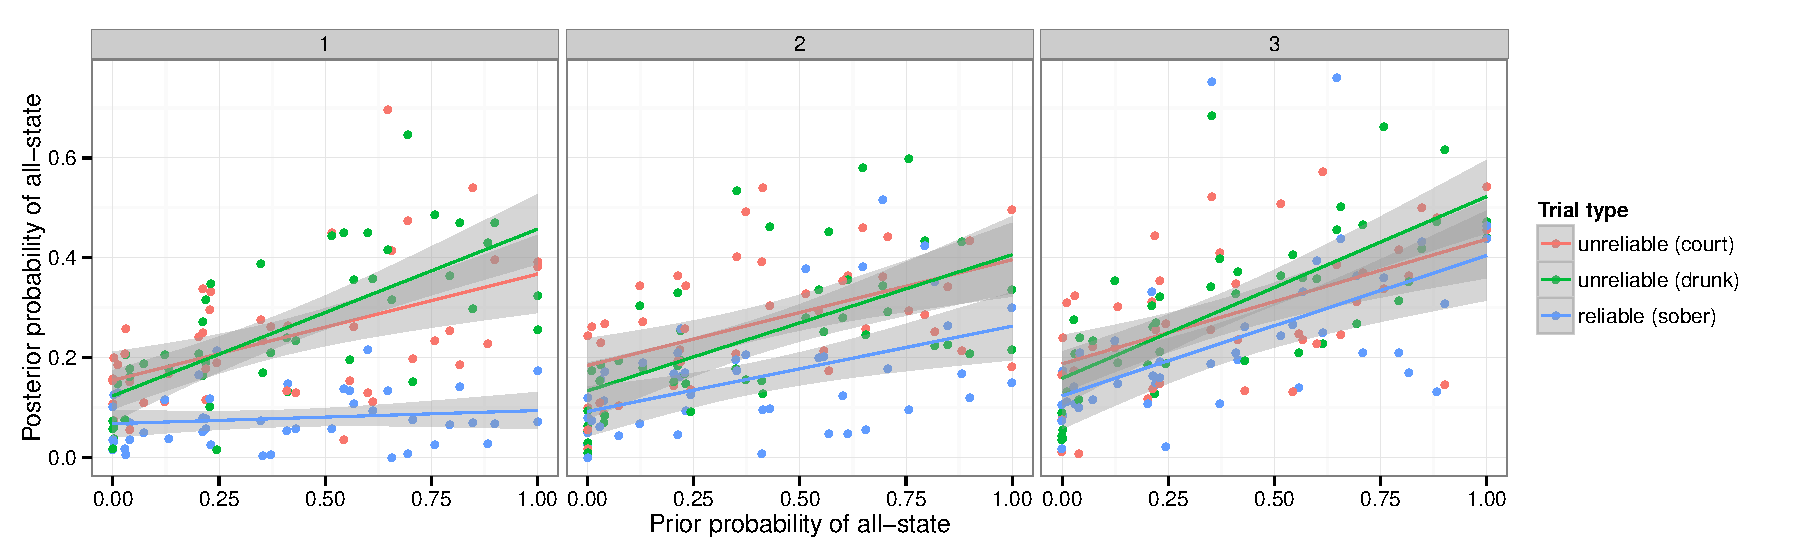
\includegraphics[width=\textwidth]{pics/speakerreliabilityresults-byblock}
%	\caption{For each item, empirical mean posterior all-state probability against  prior all-state probability for reliable (\emph{sober}) and unreliable (\emph{drunk, court}) speakers, by experimental block. Reliable speakers are increasingly treated like unreliable speakers as the experiment progresses.}
%	\label{fig:speakerreliability-byblock}	
%\end{figure}
%
  

As predicted, listeners' prior beliefs affect their interpretations more strongly when speakers are unreliable than when they are reliable.
This finding is interesting in it's own right, but also confirms that the attenuated effect of prior in Exp.~2 was unlikely to be caused by perceived unreliability of the speaker.
%In addition, as evidence for unreliability of speakers accumulates within the experiment, listeners generalize their expectation for unreliability even to \emph{a priori} reliable speakers, resulting in a greater effect of priors.

% (Intercept)                               0.2351389  0.0129339  18.180
%cAllPriorProbability                      0.2618914  0.0310649   8.430
%cReliability                              0.1137068  0.0146606   7.756
%cTrial                                    0.0031160  0.0003527   8.834
%cAllPriorProbability:cReliability         0.1408706  0.0338892   4.157
%cAllPriorProbability:cTrial               0.0037873  0.0009860   3.841
%cReliability:cTrial                       0.0002214  0.0008919   0.248
%cAllPriorProbability:cReliability:cTrial -0.0009727  0.0022225  -0.438



\section{General discussion}
\label{sec:gd}
% todo overhaul

\ndg{the discussion needs some work. i've sketched it as three main subsections below... maybe that is a good framework?}

%Interlocutors bring a wealth of world knowledge to bear on any language interpretation task. While effects of world knowledge in different areas of language processing are well-established (\red{psycholinguistics refs}), there has to date been a surprising lack of quantitative investigation into the role of world knowledge--and its defeasibility--in pragmatic inference. 
We have shown that listeners' world knowledge, in the form of prior beliefs, enters into the computation of speaker meaning in a systematic but subtle way. The effect of the prior on interpretation was much smaller, and qualitatively different, than predicted by a standard Bayesian model of quantifier interpretation (RSA). 
This suggests that in certain situations, listeners revise their assumptions about relevant priors as part of the computation of speaker meaning. 
Indeed, in the cases where the largest deviations from RSA obtained, participants also judged the world to be unusual.
%We have provided empirical evidence that the types of situations that lead to such revision , that is, situations in which the speaker's utterance is too unlikely given the listener's default prior beliefs and the available utterance alternatives. are cases of `wonky' worlds
Extending RSA with a lifted ``wonkiness'' variable that captures precisely whether listeners think the world is unusual, and allows them to back off to a uniform prior (i.e., ignore entirely their previously held beliefs about the world), provided a good fit to the empirical wonkiness judgments and dramatically improved the fit to participants' comprehension data. This model constitutes the first attempt to explicitly model the quantitative effect of world knowledge and its defeasibility on pragmatic utterance interpretation. This work raises many interesting questions, some of which we discuss in the following.

\subsection{What is wonky?}
\label{sec:whatiswonky}

In one sense the revision of beliefs in the wRSA listener is standard Bayesian belief updating with respect to a complex prior \red{insert refs that also do this}; however it is not the simple belief update of a flat or hierarchical prior, because the different aspects of prior belief (i.e.~$P(w)$ and $P(s|w)$) interact in complex ways with the listener's assumptions about the speaker.
As a result, an odd utterance can lead the listener to update their own view of $w$; this in turn impacts both their own prior over states and what prior they believe the speaker believes they are using---an odd utterance leads the listener to re-evaluate common ground. 

Throughout this paper we discussed wonkiness as an attribute of the \emph{world}, yet empirically we elicited wonkiness judgments about the \emph{objects} involved in the events. 
This raises the question of what exactly listeners are revising their prior beliefs about: objects, events, the speaker's beliefs, or the way the speaker uses language?  \red{SPELL OUT?}
\ndg{discuss: why does it matter? (how) does it relate to accommodation? how could you systematically build a revisable prior from a generative model?}

\ndg{In exp 3 we asked whether the objects are "normal", and treat this as a simple boolean wonky predicate. but normal  is scalar, suggesting that a more refined treatment might include a scale of wonkiness... future work.}

Relatedly, we have used a uniform prior distribution as the alternative to consider when the listener believes the world is wonky.  One could imagine various more flexible alternatives. For instance, listeners may make minimal adjustments to their prior knowledge, or alternatively, may prefer extreme priors that rationalize the utterance once they have discounted the usual priors.\red{SPELL OUT?}
%Do metaphorical interpretations draw listeners out of the wonky world? 
Future research should investigate the options listeners have available when their world knowledge must be revised to accommodate an utterance.

\subsection{Accommodation}

The revision to beliefs in common ground we have implicated here is reminiscent of linguistic theories of presupposition accommodation \cite{lewis1979,stalnaker1973,stalnaker1998}: in the same way that the possessive NP \emph{my cat} can trigger an accommodation process to the effect that the proposition  \emph{the speaker has a cat} is added to common ground in order to render the observed utterance felicitous, so listeners sometimes update the prior belief distribution over event types presumed to be in common ground in order to render the observed utterance felicitous. In \citeA{beaver2007}'s words:  ``we accommodate whatever seems most appropriate to make sense of the speaker's intentions in light of our joint communicational goals'' (p.~4). Here we treated the communicational goal as utility-maximizing exchange of information: listeners expect speakers to produce an utterance that trades off how informative it is with respect to mutually held prior beliefs about the world, and how likely it is to be true, given those same prior beliefs. If the utterance is too unlikely to be true or too uninformative, background beliefs are updated in such a way as to increase the utterance's informativeness or the probability of it being true. 

This update is perfectly analogous to traditional presupposition accommodation, whereby ``if the presumption of cooperative speech requires that the speaker be taking something to be common ground, $[$\dots$]$ then it is reasonable for the addressee to take the speaker to be taking it to be common ground, and if the addressee is also willing to accept it, then he too will take it to be common ground, in which case it will be common ground'' \cite[p.~540]{stalnaker2008}. Within the wonky RSA model outlined here, that ``something'' that the listener is taking the speaker to be taking to be common ground is the alternative prior on worlds. Note the following subtlety, though: in our implementation of the model, the listener's final interpretation is a mixture of wonky and non-wonky speaker meaning computations weighted by the wonkiness prior. Thus our recurring skeptical reader may point out that in fact, common ground is not updated in such a way as to fully accommodate the updated prior, since  the listener's resulting interpretation will still rely on the empirical prior to some degree. That is, in contrast to the standard view of accommodation, the listener does not categorically update their prior beliefs (or fail to do so), and thus the analogy to standard accommodation is more tenuous than it may at first blush seem. In response, we would like to propose that what is accommodated is not the update of the prior itself, but precisely the mixture of empirical and backoff prior. Indeed, in \sectionref{sec:whatiswonky} we discussed the idea that wonkiness may turn out to be better thought of as a scalar property rather than a Boolean one, in which case the accommodated information would correspond to the inferred \emph{degree} to which the world is wonky. 

It is important to note that there are some differences between our approach here and accounts of presupposition accommodation that precede us. In particular, previous accounts typically assume that there are explicit lexical items that trigger accommodation, e.g., possessives. In contrast, we treat the update of the prior as resulting from the overall oddness of the utterance in the absence of the prior update, rather than from the presence of a particular lexical item in our \emph{Q of the X Yed} utterances. However, this isn't a categorical difference between accounts. In fact, the case where lexical items like possessives trigger presupposition accommodation may just be a special case of the mechanism we're proposing:  \emph{my cat is sick} is a very odd utterance under the background belief that the speaker doesn't have a cat, not because of anything special about the possessive, but because the utterance would simply not receive a truth value if the presupposition is not accommodated.  Future research should investigate the extent to which lexically triggered accommodation processes can be accounted for in the same way we have proposed here.

\ndg{should expand discussion of accommodation, probably make into its own subsection. discuss a bit more previous proposals, and how ours differs (eg no triggers). maybe do a simple simulation of a standard accommodation example? describe briefly future work to explore presupposition and accommodation more generally.}\jd{should we discuss the fact that there are differences in whether accommodation is \emph{necessary} for the utterance to be even mildly interpretable? ie if i refuse to accommodate that john has a cat, i won't be able to get a truth value for ``my cat is sick'', but if i refuse to update my prior about sinking marbles, i can still get a truth value for ``some of the marbles sank'', my resulting beliefs about the world just probably won't be as close to the speaker's as they could or should be. i think beaver and zeevat (and probably others before them) call this the difference between semantic and pragmatic accommodation.}

\subsection{Methodological implications}

This work also has methodological implications: researchers working in the field of experimental semantics and pragmatics would be well served to take into account the effect of `odd' items, prior beliefs, and interactions between the two.\footnote{For an in depth discussion of this issue in syntactic processing, see, e.g., \citeA{jaeger2010, fine2013a}.} \red{instead of a footnote, discuss this in more detail, and as a theoretical point about how people should update their beliefs. give it a kleinschmidt spin, i.e.~what does this mean for \emph{learning}? short term (local) vs long term (global) belief update. do i infer sth about marbles in general or just the ones in this situation?} In particular, if the attempt to design uniform stimuli across conditions yields odd utterances in some conditions, we predict that participants will respond by revising their prior beliefs in ways that can be unpredictable. That is, we expect unpredictable interaction effects between stimuli and conditions. This is likely to inflate or compress potential effects of an experimental manipulation. 
\ndg{expand this point into its own subsection too: be a bit more explicit about both previous work pointing out this effect, paradigms that are particularly subject to it (ie any fully crossed pragmatics expt), and what to do about it (measure and model oddness?).}

\section{Conclusion}

\ndg{revise conclusion after revising discussion above...}
Concluding, this work exemplifies the importance and utility of exploring the detailed quantitative predictions of formal models of language understanding.
Exploring the effect of prior knowledge predicted by various models within the RSA framework has allowed us to  better understand the way in which world knowledge enters into the pragmatic interpretation of language.
Listeners have many resources open to them when confronted with an odd utterance, and, rather than giving up the assumption of speaker cooperativity, re-construing the situation in common ground appears to be a favorite.

\ndg{acknowledgements. grants: mcdonnell, ONR. snf}

\section{Acknowledgments}

This work was supported in part by a James S. McDonnell Foundation Scholar Award (to N.D.G.), Office of Naval Research Grant N000141310788 (to N.D.G.), a Swiss National Science Foundation Early Postdoc.Mobility fellowship (to J.D.), and an NSF Graduate Fellowship (to M.H.T.).

%\begin{itemize}
%
%%	\item what is wonky? -- objects, event, speaker? -- connection to adaptation?
%%	\item other ways of asking about wonkiness
%%	\item \red{what's the right prior to back off to?}
%%	\item revising private beliefs vs revising common ground.
%%	\item \red{connection to presupposition (cf stalnaker), and other phenomena}
%%	\item implication for experiments on language understanding
%
%\end{itemize}

\appendix

\section{Items}
\label{sec:items}

Items in Exps.~1 - 3 began with a \emph{context sentence} of the form \emph{CHARACTER did Z to X.} In Exps.~2 - 3, the context sentence was followed by a speaker utterance sentence of the form \emph{SPEAKER, who observed what happened, says: UTTERANCE}. On target trials, UTTERANCE was of the form \emph{QUANTIFIER of the X Yed}, where QUANTIFIER was one of \emph{some}, \emph{none}, or \emph{all}. On short filler trials, UTTERANCE was one of \emph{Typical}, \emph{Nothing out of the ordinary}, \emph{As usual}, \emph{Pretty normal}, or \emph{Nothing surprising there}. On long filler trials, UTTERANCE was customized to the particular item in such a way that the utterance addressed an aspect of the situation that was not the number of X that Yed. In the following, we list Z, X, and Y for each of the 90 items as well as its customized filler. We organize items by verb Y, since each verb shared three X and one long filler. CHARACTER and SPEAKER were randomly sampled from a list of 110 names (half male, half female) on each trial. The first 15 items were also used in Exp.~4.

\begin{enumerate}
	\item \emph{Y}: melted, \emph{X}$_1$: pencils, \emph{X}$_2$: crayons, \emph{X}$_3$: ice cubes, \emph{Z}: left in the hot sun\\
	\emph{Filler}: It's a beautiful day.
	\item \emph{Y}: stuck to the wall, \emph{X}$_1$: baseballs, \emph{X}$_2$: cakes, \emph{X}$_3$: pieces of gum, \emph{Z}: threw against a wall\\
	\emph{Filler}: What a strange thing to do.
	\item \emph{Y}: burned, \emph{X}$_1$: rocks, \emph{X}$_2$: books, \emph{X}$_3$: matches, \emph{Z}: threw into a fire\\
	\emph{Filler}: I love watching fires.
	\item \emph{Y}: blew away, \emph{X}$_1$: backpacks, \emph{X}$_2$: hats, \emph{X}$_3$: napkins, \emph{Z}: left on a table on a windy day\\
	\emph{Filler}: I just wish the weather was better.
	\item \emph{Y}: ripped, \emph{X}$_1$: shoes, \emph{X}$_2$: shirts, \emph{X}$_3$: books, \emph{Z}: used as dog toys\\
	\emph{Filler}: Doesn't the dog have its own toys?
	\item \emph{Y}: broke, \emph{X}$_1$: logs, \emph{X}$_2$: boxes, \emph{X}$_3$: sunglasses, \emph{Z}: ran over with a car\\
	\emph{Filler}: Why does Lucy always leave her stuff in the driveway?
	\item \emph{Y}: exploded, \emph{X}$_1$: candles, \emph{X}$_2$: fireworks, \emph{X}$_3$: gas tanks, \emph{Z}: lit \\
	\emph{Filler}: Who came up with that idea?
	\item \emph{Y}: dissolved, \emph{X}$_1$: carrots, \emph{X}$_2$: oreos, \emph{X}$_3$: sugar cubes, \emph{Z}: put in a bucket of water\\
	\emph{Filler}: There are people starving in the world.
	\item \emph{Y}: stuck, \emph{X}$_1$: beads, \emph{X}$_2$: sequins, \emph{X}$_3$: stickers, \emph{Z}: glued to a piece of paper\\
	\emph{Filler}: It looks like a zebra.
	\item \emph{Y}: ate the seeds, \emph{X}$_1$: dogs, \emph{X}$_2$: butterflies, \emph{X}$_3$: birds, \emph{Z}: left seeds out for\\
	\emph{Filler}: I wish someone would leave seeds out for me.
	\item \emph{Y}: landed flat, \emph{X}$_1$: notebooks, \emph{X}$_2$: pancakes, \emph{X}$_3$: coins, \emph{Z}: tossed\\
	\emph{Filler}: I love throwing stuff, too.
	\item \emph{Y}: sank, \emph{X}$_1$: balloons, \emph{X}$_2$: cups, \emph{X}$_3$: marbles, \emph{Z}: threw into a pool\\
	\emph{Filler}: It's just fun to throw stuff in the water.
	\item \emph{Y}: fell down, \emph{X}$_1$: shelves, \emph{X}$_2$: block towers, \emph{X}$_3$: card towers, \emph{Z}: punched\\
	\emph{Filler}: Some people just love destruction.
	\item \emph{Y}: rolled, \emph{X}$_1$: toy cars, \emph{X}$_2$: shopping carts, \emph{X}$_3$: wheelchairs, \emph{Z}: pushed\\
	\emph{Filler}: Pushing stuff is so much fun.
	\item \emph{Y}: froze, \emph{X}$_1$: bottles of hand soap, \emph{X}$_2$: chocolate bars, \emph{X}$_3$: berries, \emph{Z}: put in the freezer\\
	\emph{Filler}: That reminds me I need to visit my grandma.
	\item \emph{Y}: flashed, \emph{X}$_1$: webcams, \emph{X}$_2$: phones, \emph{X}$_3$: cameras, \emph{Z}: took a picture with\\
	\emph{Filler}: Everyone with the selfie craze these days.
	\item \emph{Y}: popped, \emph{X}$_1$: eggs, \emph{X}$_2$: balloons, \emph{X}$_3$: bubbles, \emph{Z}: poked with a pin\\
	\emph{Filler}: That requires a lot of concentration.
	\item \emph{Y}: exploded, \emph{X}$_1$: CDs, \emph{X}$_2$: balls of tin foil, \emph{X}$_3$: eggs, \emph{Z}: heated up in a microwave\\
	\emph{Filler}: That's one way of spending your free time.
	\item \emph{Y}: lit up, \emph{X}$_1$: cd-players, \emph{X}$_2$: computers, \emph{X}$_3$: flashlights, \emph{Z}: pressed the `on' button on\\
	\emph{Filler}: I wish we could just say `on'.
	\item \emph{Y}: beeped, \emph{X}$_1$: houses, \emph{X}$_2$: old cars, \emph{X}$_3$: new cars, \emph{Z}: left the lights on in\\
	\emph{Filler}: That's not very good for the environment.
	\item \emph{Y}: decomposed, \emph{X}$_1$: soda cans, \emph{X}$_2$: pinecones, \emph{X}$_3$: banana peels, \emph{Z}: put in a compost pile for a month\\
	\emph{Filler}: What a great way to reduce trash.						\item \emph{Y}: honked, \emph{X}$_1$: bicyclists, \emph{X}$_2$: bus drivers, \emph{X}$_3$: taxi drivers, \emph{Z}: cut off\\
	\emph{Filler}: That looks kind of dangerous.
	\item \emph{Y}: laughed, \emph{X}$_1$: lawyers, \emph{X}$_2$: comedians, \emph{X}$_3$: kids, \emph{Z}: told a joke to\\
	\emph{Filler}: I guess once a jokester, always a jokester.
	\item \emph{Y}: ran out of batteries, \emph{X}$_1$: phones, \emph{X}$_2$: bike lights, \emph{X}$_3$: laptops, \emph{Z}: left on (and unplugged) all day\\
	\emph{Filler}: That would be a pretty useful gadget.
	\item \emph{Y}: had the letter Z in them, \emph{X}$_1$: birthday cards, \emph{X}$_2$: love notes, \emph{X}$_3$: novels, \emph{Z}: wrote\\
	\emph{Filler}: I just don't have the patience to write one of those.
	\item \emph{Y}: were green, \emph{X}$_1$: strawberries, \emph{X}$_2$: bananas, \emph{X}$_3$: clovers, \emph{Z}: saw\\
	\emph{Filler}: I should start growing those myself.
	\item \emph{Y}: got stained, \emph{X}$_1$: white tablecloths, \emph{X}$_2$: white shirts, \emph{X}$_3$: white carpets, \emph{Z}: spilled red nail polish on\\
	\emph{Filler}: Why always the red?
	\item \emph{Y}: reflected the sunlight, \emph{X}$_1$: phone screens, \emph{X}$_2$: diamonds, \emph{X}$_3$: mirrors, \emph{Z}: placed in the sun\\
	\emph{Filler}: Why not just take them inside?
	\item \emph{Y}: rhymed, \emph{X}$_1$: poems, \emph{X}$_2$: songs, \emph{X}$_3$: limericks, \emph{Z}: wrote\\
	\emph{Filler}: It's so pretty.
	\item \emph{Y}: stopped, \emph{X}$_1$: bicycles, \emph{X}$_2$: motorcycles, \emph{X}$_3$: cars, \emph{Z}: pressed the brakes on\\
	\emph{Filler}: So many parts need to work for us to not die.
					 
\end{enumerate}


\section{Alternate four-step prior elicitation procedure}
\label{four-step-priors}

In order to increase our confidence in the prior belief distributions elicited in Exp.~1, we implemented an alternative prior elicitation procedure described \citeA{Speirs-Bridge2010}. We elicited participants' beliefs in four steps:\footnote{This experiment can be viewed at \url{http://cocolab.stanford.edu/cogsci2015/wonky/prior_fourstep/sinking-marbles.html}}  first, they were asked to provide a lower bound on how many marbles sank. Then they were asked to provide an upper bound. Next, they were prompted for their best guess as to how many marbles sank. All three of these estimates were given by typing a number into a text field. Finally, they were asked to rate how confident they were that the interval they created captured the actual number of marbles that sank, by adjusting a slider with endpoints labeled ``not confident at all'' and ``very confident''. A full example of questions asked is provided in \eref{fourstep}.

\eenumsentence{\label{fourstep}
				\item \emph{Realistically, what do you think the lowest number of marbles that sank could be?}
				\item \emph{Realistically, what do you think the highest number of marbles that sank could be?}
				\item\label{bestguess} \emph{Realistically, what is your best guess at how many marbles sank?}
				\item \emph{How confident are you that the interval you created, from lowest to highest, will capture the actual number of marbles that sank?}}


We were most interested in participants' response to \eref{bestguess}, which most closely matches the measure used in Exp.~1. We subjected the distributions of best guesses to the same smoothing procedure described in \sectionref{sec:priors} and computed the expected value and all-state probability for each item, visualized in \figref{fig:probhist-fourstep}. These distributions were very similar to those obtained in Exp.~1. 

\begin{figure}
\centering
	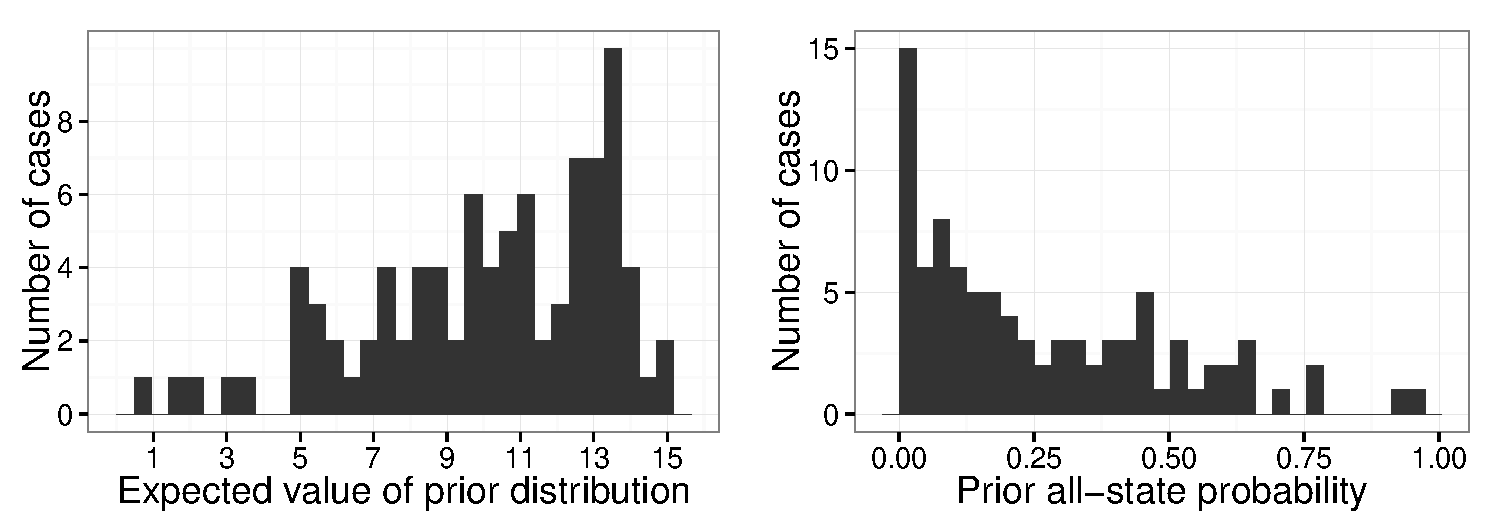
\includegraphics[width=\textwidth]{pics/priordistributions-fourstep}	
	\caption{Histogram of expected values $\mathbb{E}[P(s)]$ of each empirically elicited and smoothed prior distribution (left) and histogram of prior probabilities $P(s_{15})$  of the all-state for each item (right), using the four-step procedure.}
	\label{fig:probhist-fourstep}	
\end{figure}


\section{Bayesian model selection and comparison}
\label{app:bayesianselection}

We model the data for Experiments 2a, b, and 3 jointly.  

\subsection{Linking functions}

To compute $P(D\mid M)$, linking assumptions between the model's posterior distribution and participants' response data must be made explicit. 

\subsubsection{Experiment 2}

For Expt.~2, the (w)RSA model's posterior support consists of exact numbers of objects displaying the effect (i.e. the number of Xs that Yed). 

Experiment 2a uses a dependent measure of a number between 0 - 15. Thus, for Expt.~2a, the probability of a data point given the model --- $P(d \mid m)$ --- is simply the posterior probability from the (w)RSA model of the particular state that the participant's response is indicating. 

Experiment 2b uses a dependent measure of a slider bar rating between 0 - 1, corresponding to the probability of the ``all'' state. Thus, $P(d \mid m)$ cannot be computed  directly from the (w)RSA models because these models define a distribution over states, whereas this dependent measure is of a \emph{confidence}, or \emph{probability} of a particular state (i.e. the ``all'' state). To connect the posterior probability of the (w)RSA models to the slider bar response format, we transform the posterior probability into real space ($-\infty, \infty$) using the logit transform $g(p) = log(\frac{p}{1-p})$. We assume participants' responses are sampled from a Gaussian distribution centered at the logit-transformed posterior probability $d \sim N(g(p), \sigma)$, with unknown variance. To convert back into a response format in $[0, 1]$ (i.e. the slider bar space), we use the logistic function parametrized by scale and offset parameters: $k$ and $x_0$. 

$$ f(x) = \frac{1}{1+e^{-k(x-x_0)}}$$ 

The scale parameter $k$ intuitively corresponds to participants' \emph{sensitivity} in using the slider bar. In other words, it is the scale factor by which a change in subjective-probability space translated to the slider bar. If $0<k<1$, responses will be compressed in such a way as to avoid the endpoints of the scale (e.g. the difference between a posterior probability of 0.8 and 0.9 will translate to a difference in slider bar ratings less than 0.1).  If $k>1$, responses will be endpoint-seeking (as opposed to endpoint avoiding); this would be appropriate when small changes in probability correspond to categorical shifts in responses. When $k<0$, the slider bar reverses such that an increase in subjective probability corresponds with a \emph{decrease} in slider bar rating. Given the nature of the task and pilot experiments, we expect $0<k<1$. 

The offset parameter $x_0$ corresponds to participants' \emph{bias} when using the slider bar. In other words, if the participant wanted to give a particular response (e.g. 0.4), this is how far and in what direction the participants' response would miss their target. Another interpretation of the offset parameter is how much participants avoid one of the endpoints. For Expt.~2b, participants' data for each item is normalized to form a distribution; this may result in an overall bias away from the extreme high endpoint. The offset parameter accounts for this.

\subsubsection{Experiment 3}

For Expt.~3, the wRSA model's posterior support is a Bernoulli support. Expt.~3 uses a two-alternative, forced choice (2AFC) dependent measure corresponding to if the objects under discussion are normal or not. Hence, like Expt.~2a, we can compute the posterior probability directly from the wRSA model. 

\subsection{Posteriors over parameters}

The full data analysis model predicting data from 3 experiments (Expt.~2a, 2b, 3) has 6 parameters.


\subsection{Model comparison}

To assess whether the added complexity of the wonky RSA (wRSA) model is warranted by its predictive accuracy, we compare it to the regular RSA using a hierarchical modeling approach \cite<e.g.>{Lee2011}. That is, RSA is considered a special case of wRSA for when the wonkiness prior equals exactly 0. A Bayesian approach to model comparison adequately balances predictive accuracy with model complexity \cite{Jeffreys1961, Vandekerckhove2015}.


%\section{Sketch of proof for asymmetry in wonkiness probability}
%
%We want to know whether the asymmetric U we observe in the wonkiness probability for \emph{some} is due to the particular priors we use, or whether this asymmetry is generally predicted. Here we provide a sketch of a proof that the asymmetry is expected. \red{IN THE END WE MAY JUST GET RID OF THIS AGAIN?}
%
%The asymmetric U comes out in the most basic model that contains no linking functions or additional parameters. It makes intuitive (and formal) sense, which you can see by computing the speaker utterance distribution for each world state,  then re-weight by prior, then marginalize over states and re-normalize to get the global probability for a particular utterance FOR THAT ITEM):  
%
%\begin{equation}
%P(u) = \frac{\sum\limits_{t \in T}^{} P(t)\cdot P(u|t)}{\sum\limits_{u' \in U}^{} \sum\limits_{t \in T}^{} P(t)\cdot P(u'|t)}
%\end{equation}
%
%...assuming that T is the set of world states t0, t1, t2, t3, t4 (ie 4 instead of 15 total marbles, for simplification, but it holds for the larger state space as well) and U is the set of utterances "none", "some", "all". Consider a super left-peaked and a super right-peaked prior:
%
%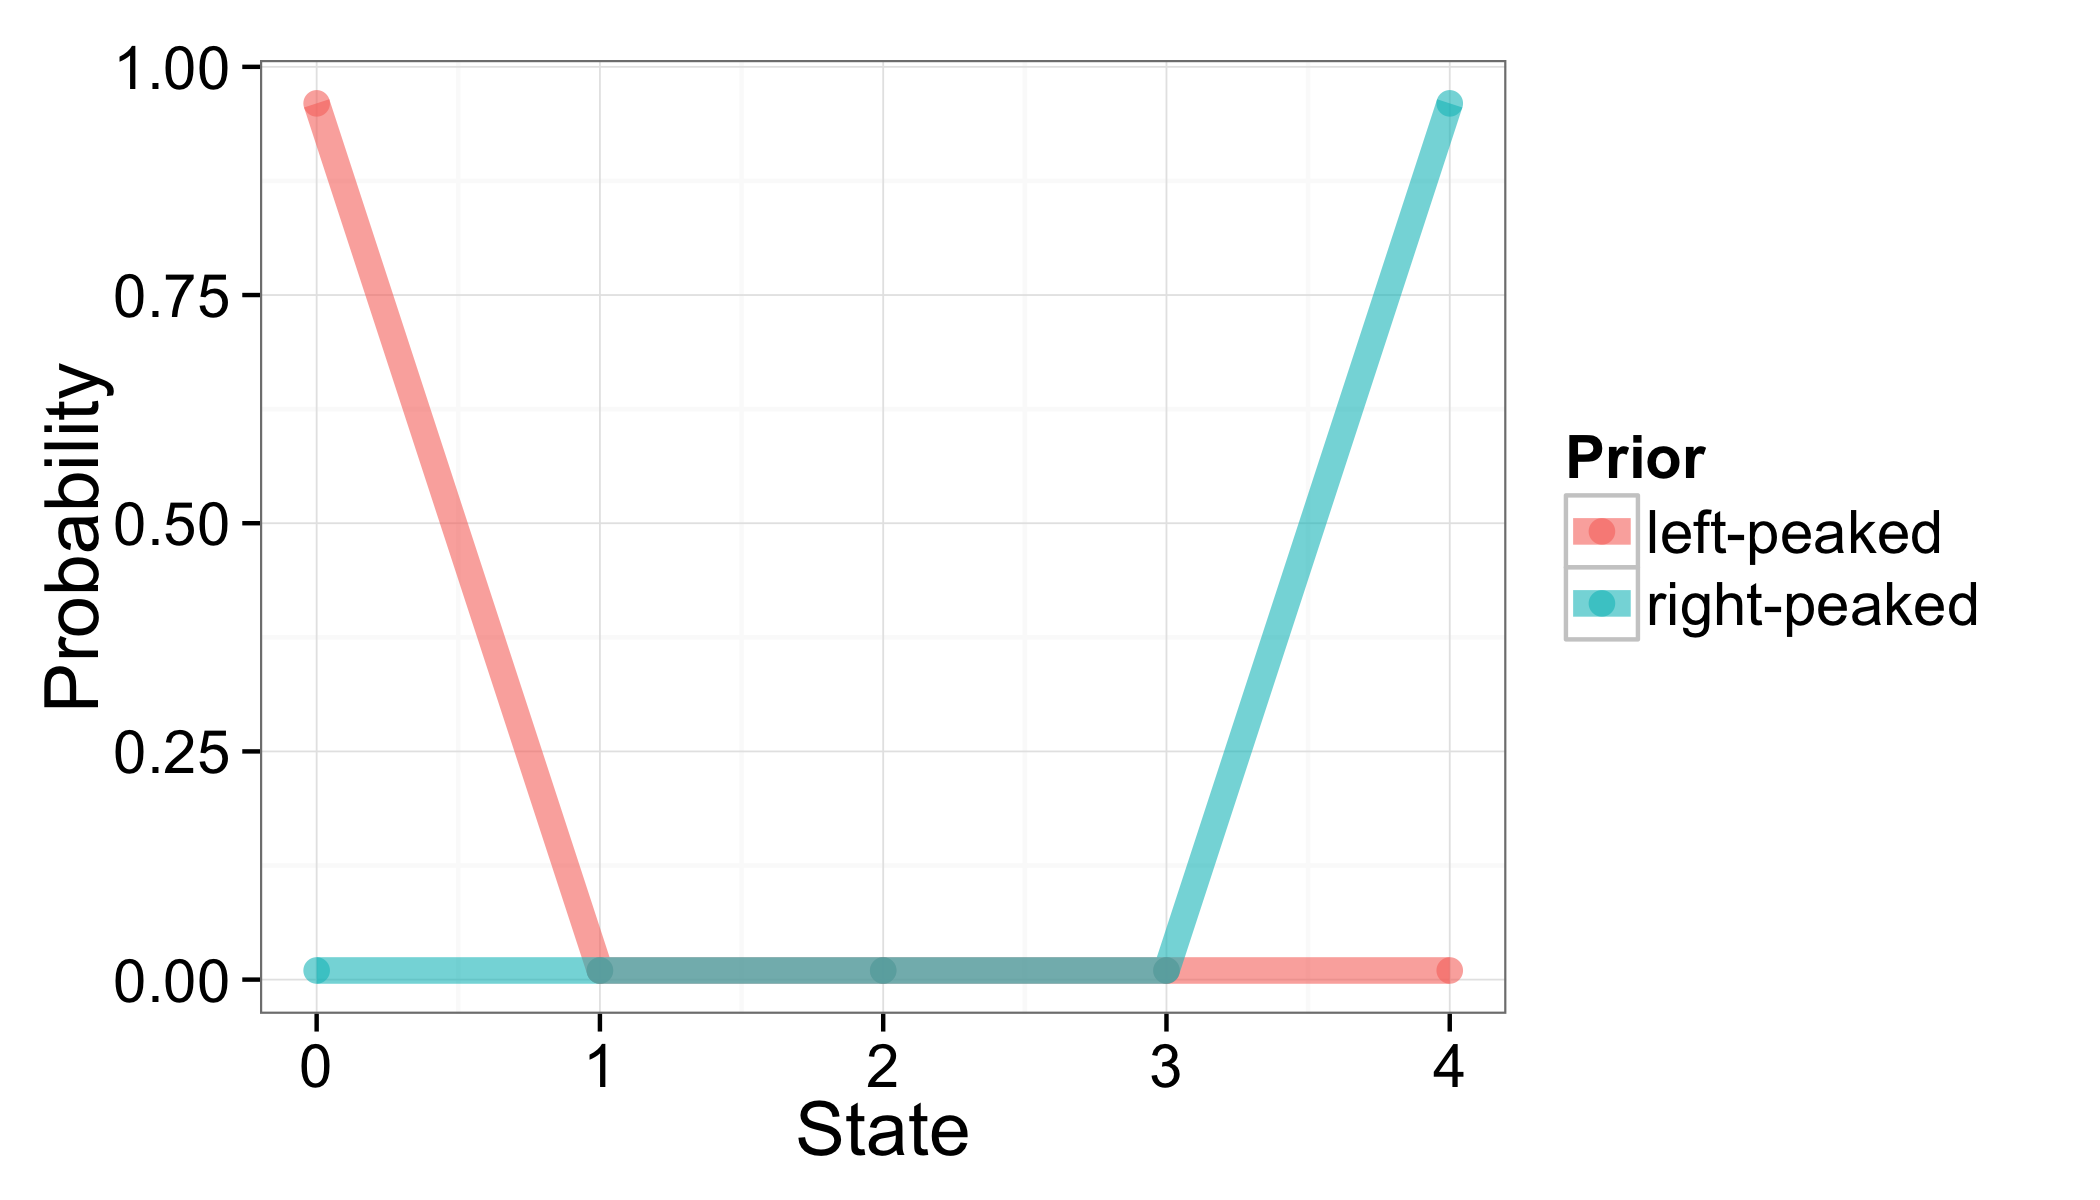
\includegraphics[width=.8\textwidth]{pics/hypothetical-priors.png}
%
%Plugging into the equation above the priors and speaker probabilities  (obtained using basic RSA, implicitly assuming a lambda of 1), we get the following overall utterance probabilities P(u):
%
%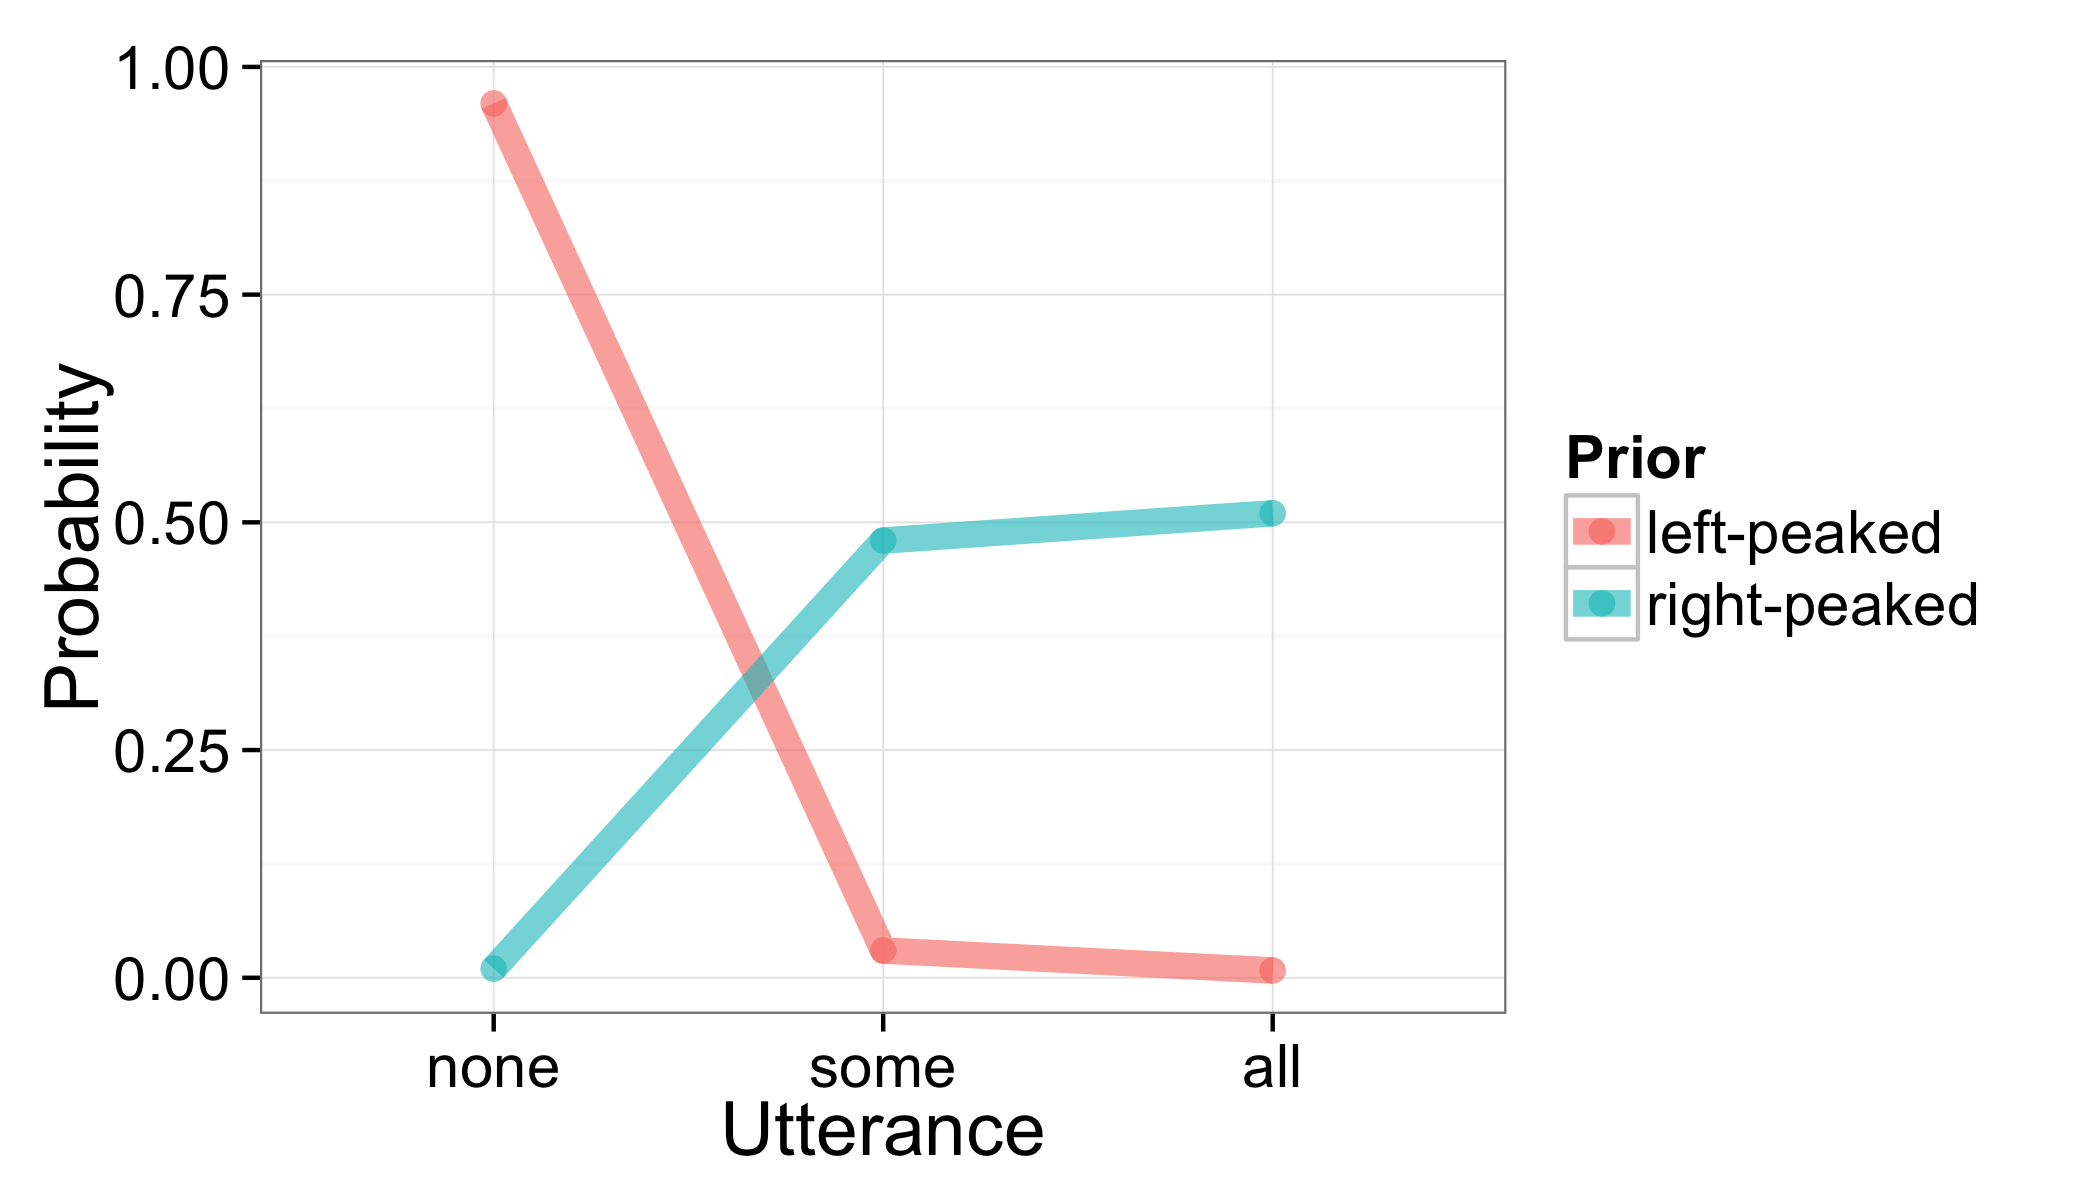
\includegraphics[width=.8\textwidth]{pics/utterance-probabilities.png}
%
%
%"some" is a more surprising utterance overall for the left-peaked items (because you only  ever expect to hear "none") than for the right-peaked items (where both "some" and "all" are semantically compatible options with the all-state). A different way of thinking about it: for the right-peaked items, whether you say "some" or "all" in the all-state doesn't matter because the prior will overwhelm interpretation anyway, so "some" is overall not too unexpected. But for the left-peaked items, whether you say "some" or "all" in the all-state really matters, because now you need pragmatic reasoning to figure out what state you're in (ie the prior won't help you distinguish the all-state from a given some-but-not-all state), so "some" is much less expected in this state, which pushes down the overall probability with which it's expected. I think this is what gives rise to the asymmetry in the extreme ends of the range of prior expected values.
%
%


\bibliographystyle{apacite}

\setlength{\bibleftmargin}{.125in}
\setlength{\bibindent}{-\bibleftmargin}

\bibliography{bibs}


\end{document}
